\documentclass{template/openetcs_report}
% Use the option "nocc" if the document is not licensed under Creative Commons
%\documentclass[nocc]{template/openetcs_article}
\usepackage{lipsum,url}
\usepackage{supertabular}
\usepackage{multirow}
\usepackage{color, colortbl}
\usepackage{hyperref}
\usepackage{listings}
\usepackage{makeidx}
\definecolor{gray}{rgb}{0.8,0.8,0.8}
\usepackage[modulo]{lineno}
\usepackage{float}
\usepackage{fixme}
\usepackage[acronym, % list of acronyms
  %section, % add the glossary to the table of content
            %description,% acronyms have a user-supplied description,
 style=longheader, % table style
 nonumberlist % no page number
  ]{glossaries}

\graphicspath{{./template/}{.}{./images/}}

\renewcommand*{\glspostdescription}{} %Deactivate point at the end of every description
\renewcommand*{\glossaryname}{Glossary}

%create glossary
 \makeglossaries
 %Glossary terms
 \loadglsentries{glossary}

\begin{document}
\frontmatter
\project{openETCS}

\newcommand{\define}[1]{\index{#1}\emph{#1}}






%Please do not change anything above this line
%============================

%user specified macros
%\newenvironment{activity}[2][planned]
	{\begin{tabular}{p{0.25\textwidth}@{\hspace{0.05\textwidth}}p{0.7\textwidth}}
			\multicolumn{2}{p{\textwidth}}{\colorbox{black}{\begin{minipage}{1.1cm}\begin{center}\textsc{\footnotesize \textcolor{white}{#1}}\end{center}\end{minipage}}~~\textbf{#2}}\\
	}
	{\end{tabular}}

\newcommand{\entry}[2]{#1:&#2\\}
\newcommand{\website}[1]{Website:&\url{#1}\\}
\newcommand{\desc}[1]{\multicolumn{2}{p{\textwidth}}{#1}\\}

\newcommand{\VV}{Verification \& Validation\xspace}
\newcommand{\vv}{verification \& validation\xspace}

\newcommand{\tbd}{\colorbox{cyan}{\%\%To Be Defined\%\%}}
\newcommand{\tbc}{\colorbox{cyan}{\%\%To Be Confirmed\%\%}}
\newcommand{\todo}[1]{\colorbox{cyan}{\%\%{#1}\%\%}}
\newcommand{\nthng}[1]{}

% The document metadata is defined below

%assign a report number here
%\reportnum{OETCS/WP3/D3.5.1.3}

%define your workpackage here
\wp{Work-Package 3: ``Modeling''}

%set a title here
\title{openETCS System Architecture and Design Specification}

%set a subtitle here
\subtitle{Third iteration: Scope of openETCS ITEA2 Functions}

%set the date of the report here
\date{November 2014}


%document approval
%define the name and affiliation of the people involved in the documents approbation here
\creatorname{Jakob G\"artner}
\creatoraffil{LEA Engineering / DB Netz}

\techassessorname{[assessor name]}
\techassessoraffil{[affiliation]}

\qualityassessorname{Izaskun de la Torre}
\qualityassessoraffil{SQS}

\approvalname{Klaus-R\"udiger Hase}
\approvalaffil{DB Netz}


%define a list of authors and their affiliation here

\author{Baseliyos Jacob, Bernd Hekele, Peyman Farhangi, Stefan Karg}

\affiliation{DB Netz AG\\
  V\"olckerstrasse 5\\
  D-80959 M\"unchen Freimann, Germany}

\author{Uwe Steinke}

\affiliation{Siemens AG}

\author{Christian Stahl}

\affiliation{TWT-GmbH}

\author{David Mentré}
\affiliation{Mitsubishi Electric R\&D Centre Europe}

\author{David Mentre}
\affiliation{Mitsubishi Electric R\&D Centre Europe}

\author{Jos Holtzer, Jan Welvaarts, Vincent Nuhaan}
\affiliation{NS}

\author{Jacob G\"artner}
\affiliation{LEA Engineering}

% define the coverart
\coverart[width=350pt]{openETCS_EUPL}

%define the type of report
\reporttype{Architecture and Functional Specification}


\begin{abstract}
%define an abstract here
This document gives an introduction to the architecture of openETCS. The functional scope is tailored to cover the functionality required for the openETCS demonstration as a target of the ITEA2 project: the Utrecht Amsterdam use-case. It has to be read as an add-on to the models in SysML, Scade and to additional reading referenced from the document.
\end{abstract}

%=============================
\maketitle

%Modification history
%if you do not need a modification history table for your document simply comment out the eight lines below
%=============================


\chapter*{Modification History}
\tablefirsthead{
\hline 
\rowcolor{gray} 
Version & Section & Modification / Description & Author \\\hline}
\begin{supertabular}{| m{1.2cm} | m{1.5cm} | m{6.6cm} | m{3.7cm} |}
0.1 & Document & Initial document providing the structure & Baseliyos Jacob \\\hline
0.2 & Document & Workshop Results included and some pretty-printing & Bernd Hekele \\\hline

\end{supertabular}

% list subsubsections in table of contents
\setcounter{tocdepth}{3}


\tableofcontents
\listoffiguresandtables
\newpage
%=============================

%Uncomment the next line if you need line numbers for tracebility when the document is in review
%\linenumbers
%=============================


% The actual document starts below this line
%=============================

\mainmatter

\chapter{Introduction}

\section{Motivation}
The openETCS work package 3 (WP3) aims to provide – amongst others - the software architecture for the openETCS kernel in order to eventually build the software itself. WP3  partner has put great effort in the openETCS software design, thus far without making definite choices on the software architecture itself respective of functional breakdown and data structures of the openETCS kernel. Since the project planning foresees in the production of a reference software to be used as a demonstrator by June 2014, it is of paramount importance that a design freeze of the openETCS kernel architecture be finalized shortly but no later than November 2014.\\

In compliance with the agreements made during the last WP 3 meeting at the 10.09.2014 in Brussels, DB has taken the initiative to design the aforesaid architecture including of functional breakdown and data structures in order to safeguard a timely delivery of these products. Furthermore, DB has ensured that these developments are focused on including end user requirements so as to develop a design in conformity with the needs and requirements of the operators. Specialists of DB and NS have cooperated together with other partners in WP3 to produce this document.\\

As referred to above, the architecture description has to be finalized in the month of November 2014. This version of the document is a draft version, demonstrating the general directions and philosophy of the architectural design, the functional breakdown of the software and the data structures. The design is focused on maximum efficiency in order to maximize on RAMS performance of the end product.\\

\textbf{This document, named second iteration, is a draft document and will be developed until a complete architecture.}\\

Since this is a work in progress, any remarks referring to the improvement of the document, including reporting errors, are more than welcome. Any additional work done thus far on the subject by other WP3 partners will be incorporated in this document as long as it is aligned with and consistent or complementary  to the fundamental viewpoints advocated in this document after a review in respect to the openETCS process. At the same time, any contributions to the  integration of which will demand discussion or changes of the fundamentals as proposed in this document, will be discarded with . Only in this way the ITEA2 project is able to meet its objectives as mentioned above. There will be two workshops in which there is due time and opportunities to fine-tune this document and its contents. Any comments will be addressed there.\\

It is urgent to definitely finalize the architecture on a short notice and therefore this document will rather prescribe than describe the openETCS architecture, functional decomposition of the system and the data structures within the limits as stated above. The document is divided in two parts, i.e.:\\
•	A description of the general architecture of the openETCS OnBoard Kernel (software) including data structures prepared by NS….\\
•	A description of the functional decomposition of the openETCS OBU (software) in alignment with the general architecture prepared by DB…..\\


Furthermore, this document describes the preconditions on which said descriptions are based on, the status and planning of upcoming activities and the main objectives of DB and NS as the End User. Wherever necessary, reference will be made to documents that underline the agreements that have been made during the openETCS architecture design process and the activities and meetings of WP3. \\


\section{Objectives}

The prime objective of WP3 is to produce a rapid prototype for the openETCS reference system that can function as a demonstrator in collaboration with WP 4 and WP 5  for the openETCS approach and will be used as such in the final phase of the project. That phase is the first half of 2015.  This objective is defined as … 

\textbf{High level Objectives of this work:}\\
<<any further general statements on the ITEA2  objectives, like…>>\\
• Work on a model bases approach and process for effective collaborative work within an international ETCS developer team
as stated above, the project needs a definite architecture design by the end of 2014.  This document targets:\\
•	Defining the general design and conditions of the openETCS architecture, functional breakdown and data structures;\\
•	Providing the guidelines for discussion during the workshops that are planned in October and November 2014 that will result in the final and decisive version of this document;\\
•	Being the ‘platform’ for finalization i.e. whatever be the products or results of the workshops shall be integrated in this document. 
Apart from these general objectives, the document means to provide for the materials that will enable WP3 partners to improve the efficiency of the Work Package activities:\\
• The comprehensive architecture design shall enable splitting the work load according to the building blocks defined by the architecture and allocate strictly compartmented work parcels or activities to WP3 partners. \\
• Doing so will enable WP3 to avoid any double work\\
• Compartmenting the work load according to the functional building blocks as defined by the architecture will enable efficient planning of activities, be it individually or the integrated WP3 planning for the coming period, aiming at a just in time delivery of all results and products;\\
• Each partner that is responsible for one of the work parcels shall abide by the requirements in terms of quality and timeliness as defined by this document and prior documents and agreements made within the ITEA2 project.\\

\section{Roles, responsibilities and tasks}
In this section, the roles and responsibilities of the WP3 partners are confirmed, especially where they divert from what has been agreed upon at the start of WP3:\\
•	First of all, in the last WP 3 meeting in Brussels on  10.09.2014 DB proposed to take over the lead of the architecture design and functional breakdown. At the subsequent weekly scrum meeting on 12.09.2014,  it was agreed upon by all participants that DB will take over the lead (see Appendix … );\\
•\textbf{Planning:} Alstom as WP 3 leader will remain to be responsible for the planning and the allocation of the defined tasks to the different partners\\
•\textbf{Roles:} Alstom will also coordinate the work and safeguard that the defined results will be delivered according to the quality requirements that are agreed within the ITEA2 project and the schedule and the milestones that will be agreed upon during the coming workshops;\\
•All WP3 partners will deliver the results or products according to planning as will be agreed upon during the said workshops. \\

In the interest of a swift production of the critical documentation of which this version is a draft, specific tasks will be defined in terms of concrete results to be delivered, the timeframes in which these results must be produced and the partner who shall be responsible for that specific result and the planning. This is to safeguard the timely delivery. The process will be described in the next sections.\\

\section{Process}
\begin{itemize}
\item Alstom as WP 3 leader will be responsible for planning
\item Time and quality aspects should be respected
\item openETCS tools and methodology must be respected
\end{itemize}

Most of the operational requirements to WP3 in the last phases of the ITEA2 project have been described in the former paragraphs. This section will describe the process which has to lead to the final result: the reference software to be used in the demonstrator next year, more specifically the final description of the openETCS architecture including the data structures and its functional decomposition. The process will run as follows:\\
•	DB will supervise  the development of the first ‘firm’ draft of the specified products, ‘firm’ meaning that changes can only be made within the framework of these products and not to the fundamentals of these products as described in this document; \\
•	DB will supervise the preparation of the two workshops that are proposed by Alstom and aim at defining the final and definite architecture, data structures and functional decomposition. It will make proposals for a planning of the critical tasks that remain to be done;\\
•	Alstom will lead the two workshops following the preparations and the instructions of DB. Since all participants are intrinsically involved in the development work and tend to immerse themselves in technical discussions, for productivity purposes it is proposed to make use of a (non-technical) moderator that will be made responsible for coordinating the meeting, the discussions and the team efforts according ot the agenda.\\
•	Also for productivity reasons, introductory presentations will be restricted to the contents and setup of this document since all prior efforts have to be merged with this document and not the other way around. Following a general introduction into the work that has been so far, the other contributions will be scrutinized on their consistency with this document and any useful sections will be merged with this document.\\
•	During the workshops, there will be ample room reserved for enhancing this document, using other documents pertaining to the same field of work that have been delivered by other partners. Only material that is aligned with the general philosophy and structures proposed by this document, will be integrated;\\
•	In case conflicting views emerge over the benefits and value of certain contributions, at the very moment that parties conclude that they have conflicting views, these will be listed in an inventory for later discussion. The moderator shall note any such conflicts on the said inventory. Conflicting views will be treated at the end of each workshop whenever there is sufficient time or will be treated in a separate meeting that will be chaired by DB as coordinator of the ITEA2 project.\\
•	The workshop shall be attended by a secretary provided for by DB who is responsible for making the workshop minutes. Within a week after each workshop these minutes shall be distributed among the partners that have cooperated in the workshop and be reviewed by those. \\
•	The main objective of the workshops shall be the finalization of this document. In order to reach the specified result, the remaining tasks shall be identified and split into separate tasks or work parcels. Every task or work parcel will be allotted to one single responsible partner. Responsibility relates to the timely delivery of the defined result and according to quality requirements;\\
•	Alstom, as WP3 leader, will be responsible for the planning, allocation of tasks or work parcels to partners and will ensure timely delivery of results;\\
•	In case there will be tasks or work packages that cannot be finalized during the workshops or will be identified during the workshops and do not fit in the actual planning, these will be allotted in such a way that deadlines are perfectly clear and acknowledged by the party that is responsible for the results, fit within the general requirements of the project and are agreed upon in writing and executed by the responsible partners according to agreement;\\
•	DB as partner that has integral responsibility for both the ITEA2 project and responsible as well for the architecture etc. , is entitled to interfere take over the role as leader / coordinator in case the workshops prove to be insufficiently productive;\\
•	All output will be such, that it can be integrated in this document. It is the responsibility of DB to integrate the results and to deliver the final and definite version of this document. \\
•	The document concept will follow the openETCS process and tools (LaTex and Git-hub).\\

\section{Assumption and Preconditions}
\begin{itemize}
\item All future contributions shall be fully aligned an compliant the finalized and approved document 
\item Alls documents produced by the partners are requested to be compliant and merge to this document; other contributions will be discarded
\end{itemize}
The workshops are all about working as swift, as efficient and as productive as possible and make full use of the potential made available for these workshops by the partners. It is expected that the partners in the workshops will have the express intention to:\\
•	Contribute to the workshops with the intention to finalize the openETCS architecture;\\
•	Provide resources according to the agreements made prior to the Workshops;\\
•	Focus primarily on  getting concrete results regardless of methodological issues that might arise. Where necessary or opportune, classical project management methodology will be applied;\\
•	Provide full transparency with respect to experience, knowledge base and information touching the subjects to be treated in the workshops;\\
•	Document on paper or electronically all output of the workshops and integrate these with the underlying document;\\
•	Restrict discussions only to topics that have an immediate impact on the content or the quality of the end product: the improved version of this document.\\


\section{Functions ERTMS/ETCS}
The ERTMS / ETCS system was developed with a view to interoperability of trains on the 
different European rail networks. It is divided into "tracks" - and "board" finishes 
and shall establish a mutual message operation, by beacons or through a "radio" - 
The transmission system (in this case a mobile telephone network GSM-R) is performed. 
It defines several operating levels, and the system must also interfaces with the 
existing monitoring systems of the trains (using \gls{STM}) have. 
The ERTMS / ETCS system provides the transport operator (the track) the choice of conditions 
concerning the use and operation. 
The train must therefore may go with different operating conditions on routes. 
Thus has the onboard equipment but must be implemented, 
to the interoperability of the train to ensure on the other networks. 
These functions must therefore correspond to one standard: the \gls{SRS} (version 3.3.0). 

application functions, which have two different species of origin: 
defined in the \gls{SRS}: here one finds in particular the 
speed monitoring- and transfer functions; these functions 
must be implemented in full accordance with the \gls{SRS}; they can in 
indeed be on any network on which the train is used; these functions 
are described below in Section \ref{SRSFunction}; 


Moreover, there are functions to adapt to the train: so, for example, the processing 
a "separation distance" in the airborne equipment trigger: 
This is dependent on the distribution of functions between the 
Control monitoring equipment (which the ERTMS / ETCS), and the other 
CCS Systems.

\section{openETCS Architecture: History and Iterations}

The openETCS Architecture and Design is implemented in iterations \cite{deployment}. The current step (second iteration) is based on a step to implement the kernel functions of the ETCS system \cite{firstIteration}. For a better understanding of the scope the Iteration is described in the following.

\subsection{First Iteration Functional Scope: The Minimum OBU Kernel Function}
\label{sec:FunctionalScopeTheMinimumOBUKernelFunction}

The openETCS first iteration architecture and the design of the openETCS OBU software as mainly specified in \cite{subset-026} UNISIG Subset\_026 version\_3.3.0. 

The appropriate functionality has been divided into a list of functions of different complexity (see the WP3 function list \cite{functions}).

All these functions are object of the openETCS project and have to be analysed from their requirements and subsequently modelled and implemented. With limited manpower, a reasonable selection and order of these functions is required for the practical work that allows the distribution of the workload, more openETCS participants to join and leads to an executable---limited---kernel function as soon as possible. 

While the first version of this document focuses on the first version of the limited kernel function, it is intended to grow in parallel to the growing openETCS software.

The first objective of the first iteration was
\begin{itemize}
	\item ``Make the train run as soon as possible, with a very minimum functionality, and in the form of a rapid prototype.''
\end{itemize}
This does not contradict the openETCS goal to conform to EN50128.
\begin{itemize}
	\item After a phase of prototyping, the openETCS software shall be implemented in compliance to EN50128 for SIL4 systems.
\end{itemize}

\subsection{How to find the functions of the First Iteration in the Architecture}
The functions will be merged with the new architecture. Wherever a function has already been in the scope it will be marked as "first iteration".

%\section{Glossary and Abbreviations}
%\glossarystyle{long}
%\printglossary[title=]


%\section{Abbreviations}
%\printglossary[type=\acronymtype,title=]

\glsaddall
\printglossaries

Missing Terms:\\
SR Staff Responsible Mode\\
SH Shunting Mode\\
%\gls{
RIU: Radio In-fill Unit\\

\section{Data dictionary}
\textbf{concept for the data dictionary ...}\\

\chapter{Input Documents}
See Wiki page on ....

\textbf{https://github.com/openETCS/modeling/wiki/Input-Documents-Repository}\\


\chapter{Product Backlog}
\textbf{See on:}\\ 


\chapter{Architecture description (by layers)}

\section{Introduction to the Architecture}

\subsection{Abstract Hardware Architecture}

For proper understanding of openETCS \gls{API} and of constraints imposed on
both sides of the \gls{API}, we need to define a \define{reference abstract hardware architecture}. This hardware architecture is ``abstract''
is the sense that the actual vendor specific hardware architecture
might be totally different of the abstract architecture described in
this chapter. For example, several units might be grouped together on
the same processor.

However the actual vendor specific architecture shall fulfil all the
requirements and constraints of this reference abstract hardware
architecture and shall not request additional constraints.

\subsection{Definition of the reference abstract hardware architecture}

\begin{figure}
  \centering
  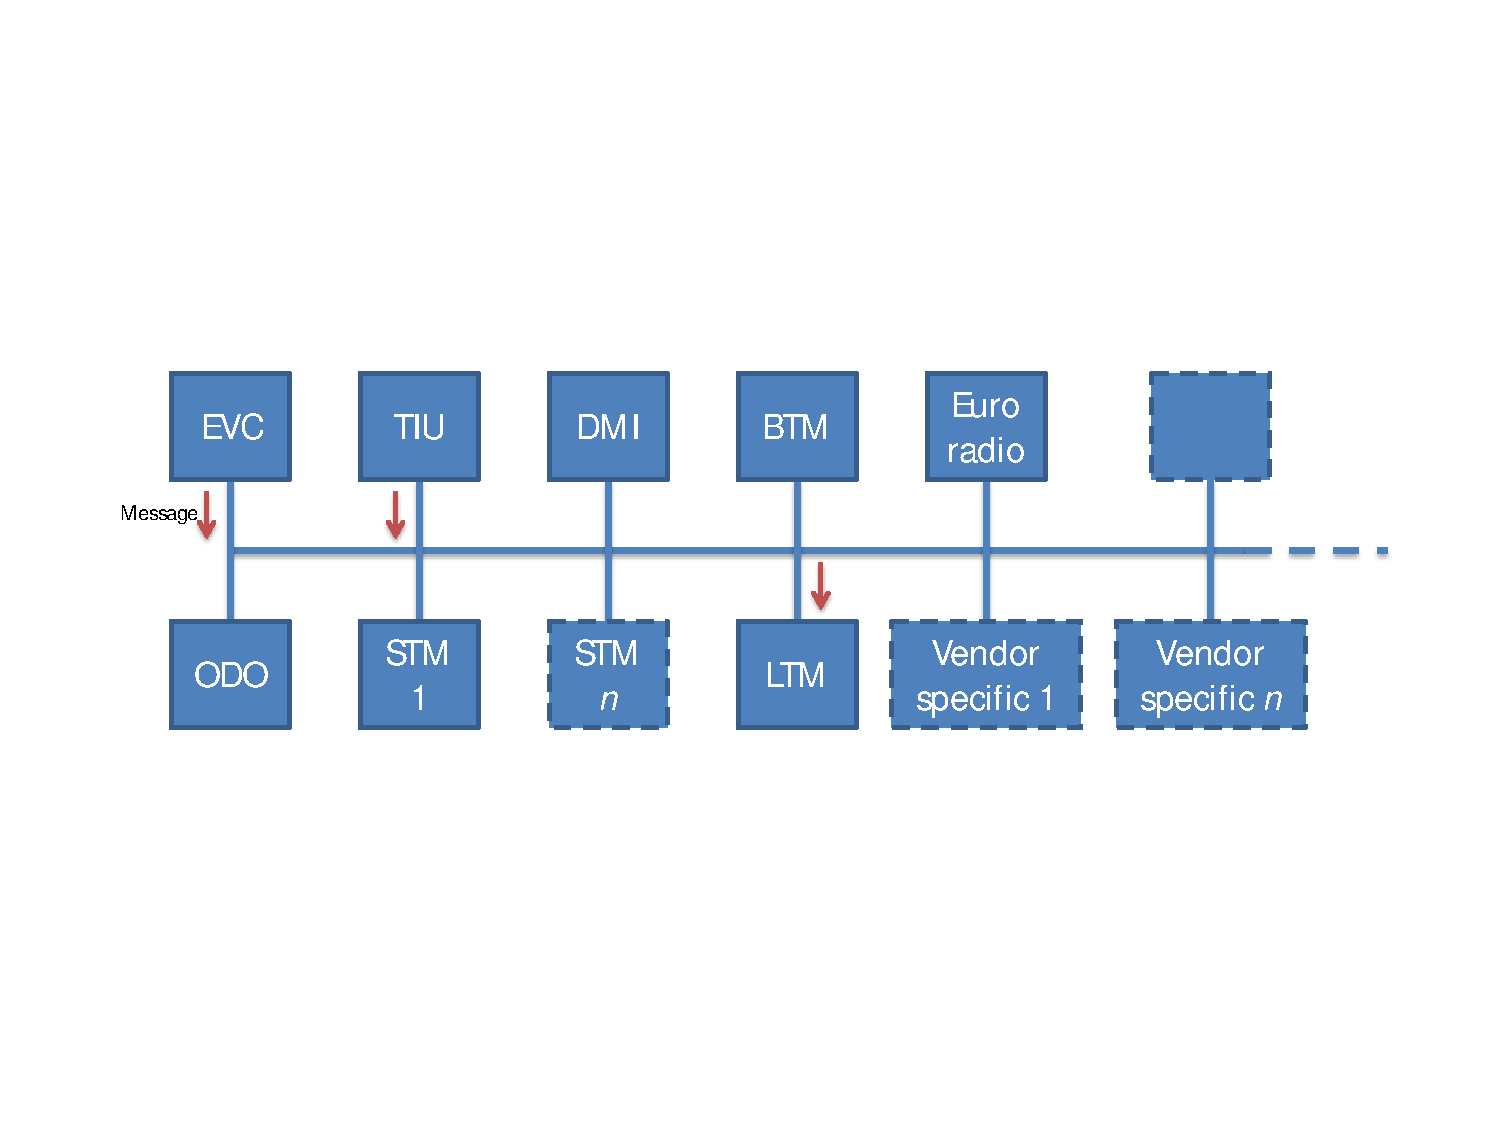
\includegraphics[width=\linewidth]{abstract-hardware-architecture.pdf}
  \caption{Reference abstract hardware architecture}
  \label{fig:hardware-arch}
\end{figure}

The reference abstract hardware architecture is shown in figure
\ref{fig:hardware-arch}.

The reference abstract hardware architecture is made of a bus on which
are connected \define{units} defining the \gls{OBU}:

\begin{itemize}
\item \gls{EVC};
\item \gls{TIU};
\item \gls{ODO};
\item \gls{DMI};
\item \gls{STM};
\item \gls{BTM};
\item \gls{LTM}: Not part of this openETCS implementation;
\item EURORADIO;
\item \gls{JRU}: Not part of this openETCS implementation;
\end{itemize}

Elements not being part of this implementation are marked. 

Those units shall working concurrently. They shall exchange
information with other units through asynchronous message passing.

\subsection{Reference abstract software architecture}
\label{software-arch}

\begin{figure}[htbp]
  \centering
  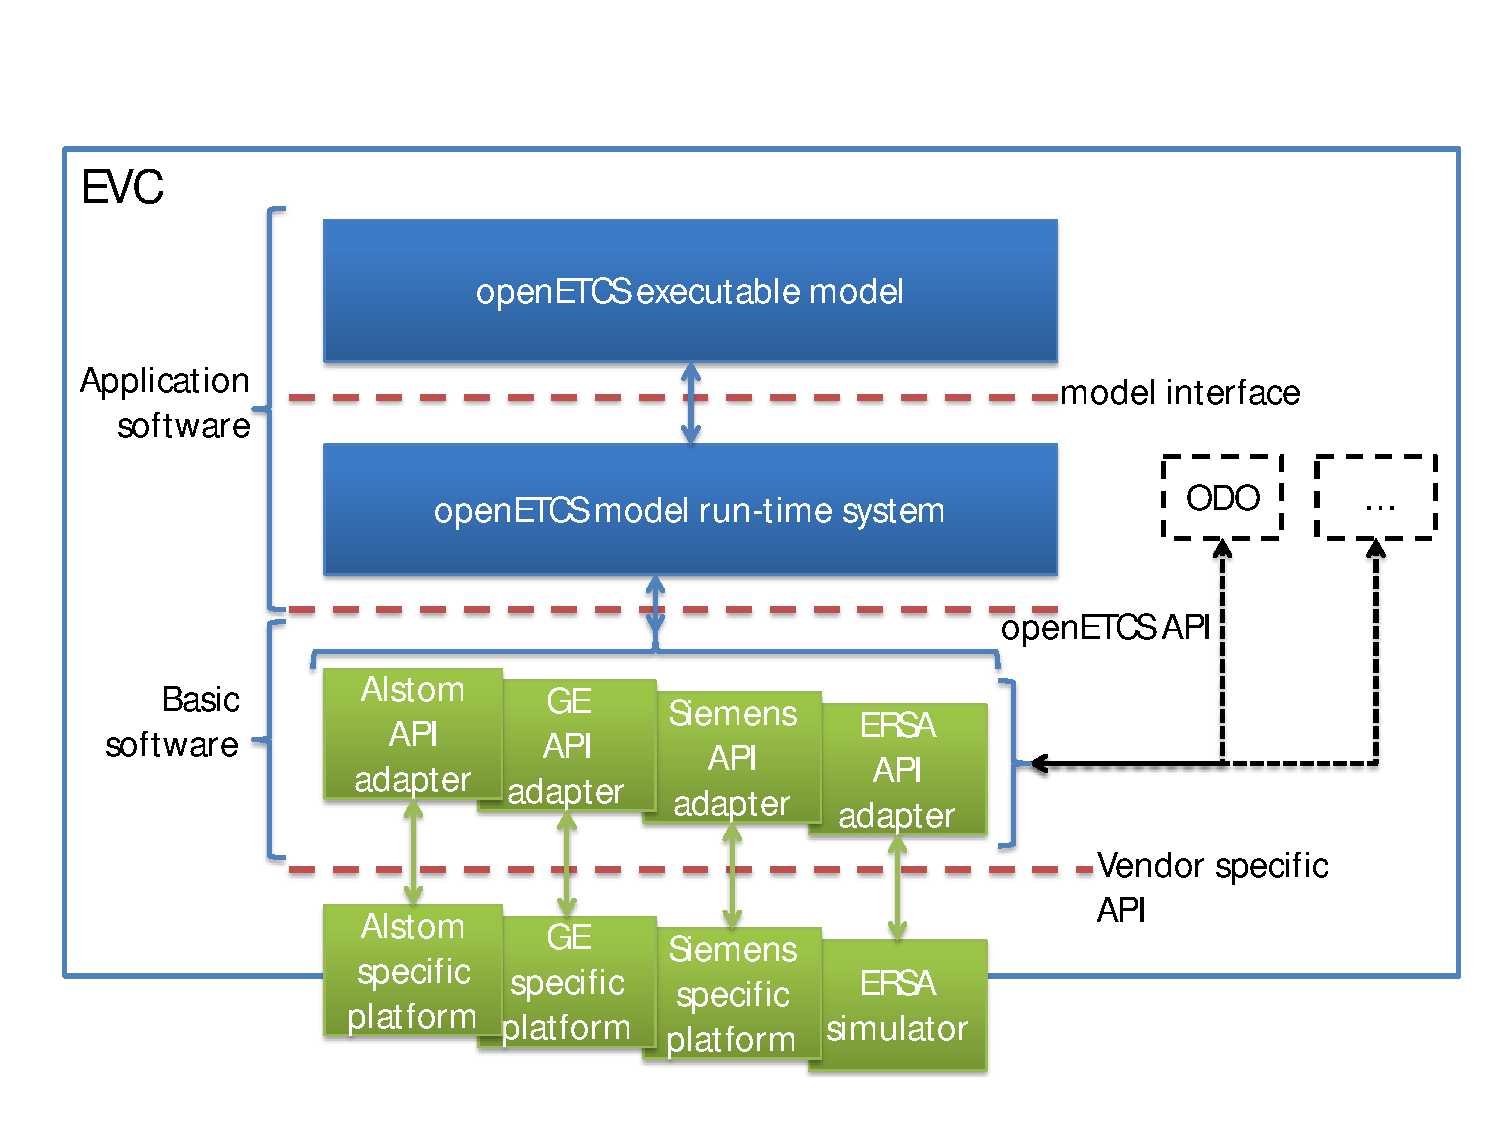
\includegraphics[width=\linewidth]{software-architecture.pdf}
  \caption{Reference abstract software architecture}
  \label{fig:software-arch}
\end{figure}

The \define{reference abstract software architecture} is shown in figure
\ref{fig:software-arch}. This architecture is made of following
elements:
\begin{itemize}
\item \define{openETCS executable model} produced by the
  \cite{scade-model} Scade Model. It shall contain the program implementing core
  ETCS functions;
\item\define{openETCS model run-time system} shall help the execution
  of the openETCS executable model by providing additional functions
  like encode/decode messages, proper execution of the model through
  appropriate scheduling, re-order or prioritize messages, etc. 
\item \define{Vendor specific \gls{API} adapter} shall make the link between
  the Vendor specific platform and the openETCS model run-time system.
  It can buffer message parts, encode/decode messages, route messages
  to other \gls{EVC} components, etc.
\item All above three elements shall be included in the \gls{EVC};
\item \define{Vendor specific platform} shall be all other elements of
  the system, bus and other units, as shown in figure
  \ref{fig:hardware-arch}.
\end{itemize}

We have thus three interfaces:
\begin{itemize}
\item \define{model interface}
 is the interface between openETCS
  executable model and openETCS model run-time system. 
\item \define{openETCS \gls{API}}
 is the interface between openETCS model
  run-time system and Vendor specific \gls{API} adapter.
\item \define{Vendor specific \gls{API}}
 is the interface between Vendor
  specific \gls{API} adapter and Vendor specific platform. This interface is
  not publicly described for all vendors. You can find the Alstom imnplementation as an example.
\end{itemize}

The two blocks openETCS executable model and openETCS model run-time
system are making the \define{Application software} part. This Application software might be either openETCS reference software or
vendor specific software.

The Vendor specific \gls{API} adapter is making the \define{Basic software} part.


\section{Functional breakdown}


\subsection{F1: openETCS \gls{API} Runtime System and Input to the EVC)}
\label{chp_openETCS_API}
%Authors: Bernd Hekele (DB)

\begin{figure}[hbtp]
\centering
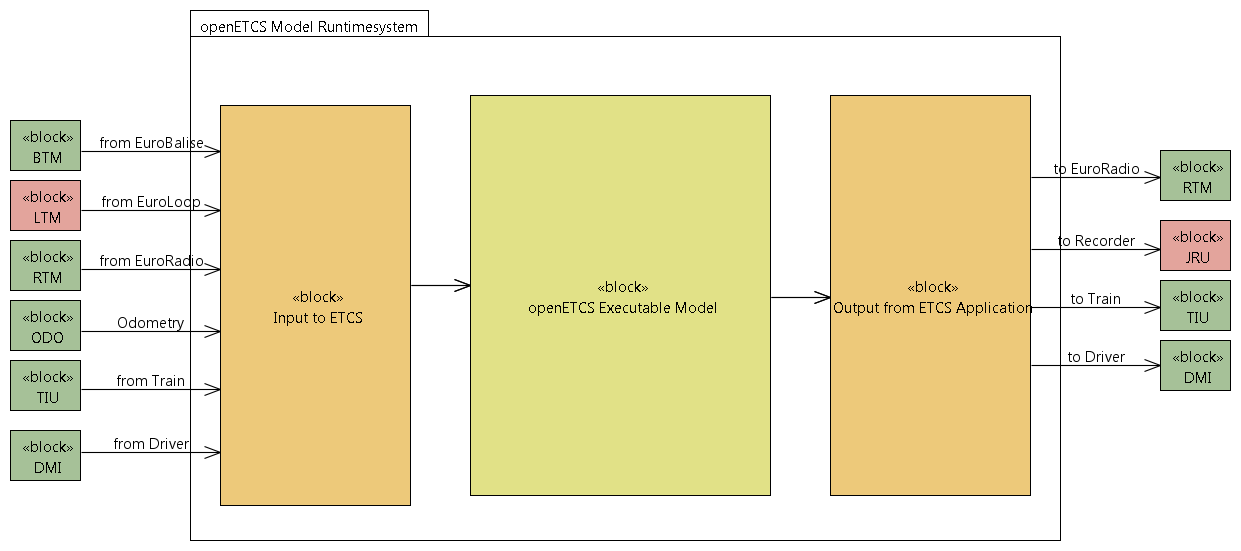
\includegraphics[width=\linewidth]{openETCSAPI.png}
\caption{openETCS API Highlevel View}
\label{fig:apiHighLevel}
\end{figure}

Figure \ref{fig:apiHighLevel} shows the structure of API with respect of the software architecture. Input boxes and output boxes not implemented in this stage are marked as red, other interfaces are marked as green. The System covers functions for processing Inputs from other Units, functions for processing Outputs to other functions and a basic runtime system. Inputs are used to feed the input to the executable model before calling it, outputs are used for collecting information provided by the executable model to be passed to the relevant interfaces after the execution cycle has finished.

\subsubsection{Principles for Interfaces (openETCS \gls{API})}

\fxnote{Version Management}
\fxnote{Layering in API + Bitwalker}
\fxnote{Mapping Input Packages inernal packages}

Information  is exchanged \define{messages} in an asynchronous way. A message is a set
of information corresponding to an event of a particular unit, e.g. a
balise received from the \gls{BTM}. The possible kind of messages are
described in chapter \ref{information-flows}.

The information is passed to the executable model as parmeters to the snychronous call of a procedure (Interface to the executable model). Since the availability of input messages to the application is not guaranteed the parts of the interfaces are defined with a "present" flag. In addition, fields of input arraysquite often is of variable size. Implementation in the concrete interface in this use-case is the use of a "size" parameter and a "valid"-flag.


\subsubsection{openETCS Model Runtime System}
The openETCS model runtime system also provides:

\begin{itemize}
\item Input Functions From other Units\\
In this entity messages from other connected units are received.
\item Output Functions to other Units\\
The entity writes messages to other connected units.
\item Conversation Functions for Messages (Bitwalker)\\
The conversion function are triggered by Input and Ouput Functions. The main task is to convert input messages from an bit-packed format into logical ETCS messages (the ETCS language) and Output messages from Logical into a bit-packed format. The logical format of the messages is defined for all used types in the openETCS data dictonary. \\
Variable size elements in the Messages are converted to fixed length arrays with an used elements indicator.\\
Optional elements are indicated with an valid flag.
The conversion routines are responsible for checking the data received is valid. If  faults are detected the information is passed to the openETCS executable model for further reaction. 
\item Model Cycle\\

The version management function is part of the message handling.This implies, conversions from other physical or logical layouts of messages are mapped onto a generic format used in the EVC. Information about the origin version of the message is part of the messages.
 
The executable model is called in cycles. In the cycle 
\begin{itemize}
\item First the received input messages are decoded
\item The input data is passed to the executable model in a predefined order. \textbf{(Details for the interface to be defined)}.
\item Output is encoded according to the \gls{SRS} and passed to the  buffers to the units.
\end{itemize}
\end{itemize}


\subsubsection{Input Interfaces of the openETCS API From other Units of the OBU}
Interfaces are defined in the Scade project APITypes (package API\_Msg\_Pkg.xscade).

In the interfaces the following principles for indicating the quality of the information is used:


\tablefirsthead{
\hline 
\rowcolor{gray} 
Indicator & Type & Purpose \\\hline}
\begin{supertabular}{| p{2 cm} | p{2 cm} | p{8 cm} |}
present & bool & True indicates the component has been changed compared to the previous call of the routine
\\\hline 
valid & bool & True indicates the component is valid to be used. 
\\\hline 
validated & bool & True indicates the component has been validated.
\\\hline 
\end{supertabular}

In the next table we can see the interfaces being used in the openETCS system. Details on the interfaces are defined further down.

\tablefirsthead{
\hline 
\rowcolor{gray} 
Unit & Name &  Processing Function & Description \\\hline}
%\begin{itemize}{| m{1.2cm} | m{1.5cm} | m{1.2cm} | m{3.7cm}  | m{3.7cm} |}
\begin{supertabular}{| c | c | c  | c |}
\gls{BTM} & Balise Telegram & Receive Messages & \\\hline
\gls{DMI} & & & \\\hline
EURORADIO & Communication Management & Communication Management & \\\hline
EURORADIO & Radio Messages & Receive Messages & \\\hline
\gls{ODO} & Odometer & All Parts & \\\hline
TIME & Time system of the OBU & All Parts & \\\hline
Startup & & & \\\hline
TIU & Train Data & All Parts & \\\hline
\end{supertabular}

Infrmation in the following sections gives an more detailed overview of the structure of the interfaces.


\subsubsection{Message based interface (BTM, RTM)}


Balise Message (Track to Train)\\

\tablefirsthead{
\hline 
\rowcolor{gray} 
Message Name & Optional Packets & Restrictions in the current scope \\\hline}
\begin{supertabular}{| p{4 cm} | p{6 cm} | p{4,5 cm} |}
Balise Telegram &
3: National Values \newline
41: Level Transition Order \newline
42: Session Management  \newline
45: Radio Network registration \newline
46: Conditional Level Transition Order \newline
65: Temporary Speed Restriction \newline
72: Packet for sending plain text messages \newline
137: Stop if in Staff Responsible \newline
255: End of Information \newline
& Used in Scenario
\\\hline
Balise Telegram &
0, 2, 3, 5, 6, 12, 16, 21, 27, 39,
40, 41, 42, 44, 45, 46, 49, 51, 52, 65,
66, 67, 68, 69, 70, 71, 72, 76, 79, 80,
88, 90, 131, 132, 133, 134, 135, 136, 137, 138,
139, 141, 145, 180, 181, 254
&  Not Used in Scenario\\\hline
\end{supertabular}

Radio Messages (Track to Train)\\
The following table gives a list of relevant messages and packets in the messages. The information is taken from track descriptions and traces.

\tablefirsthead{
\hline 
\rowcolor{gray} 
Message Name & Optional Packets & Restrictions in the current scope \\\hline}
\begin{supertabular}{| p{4 cm} | p{8 cm} | p{2,5 cm} |}
3: Movement Authority &
 21:\ Gradient\ Profile\newline
 27: International Static Speed Profile\newline
 49: List of balises for SH Area\newline
 80: Mode profile\newline
 plus common optional packets,\newline
 3: National Values \newline
 5: Linking  \newline
 15: Level 2/3 Movement Authority \newline
 21: Gradient Profile\newline
 41: Level Transition Order \newline
 65: Temporary Speed Restriction \newline
 & 
 The list of packets is adjusted to our use-case.  \\\hline
8: Acknowledgement of Train Data & &  No Extra Packets \\\hline
9: Request To Shorten MA &
 49: List of balises for SH Area\newline
 80: Mode profile\newline 
& Not part of the use-case \\\hline
15: Conditional Emergency Stop &  & No Extra Packets \\\hline
16: Unconditional Emergency Stop &  & No Extra Packets \\\hline
18: Revocation of Emergency Stop &  & No Extra Packets \\\hline
24: General Message &
From RBC:\newline
 21:\ Gradient\ Profile\newline
 27: International Static Speed Profile\newline
 plus common optional packets, e.g., for our Use-Case\newline
 3: National Values \newline
 41: Level Transition Order \newline
 42: Session Management \newline
 57: Movement Authority Request Parameters \newline
 58: Position Report Parameters \newline
 72: Packet for sending plain text messages \newline
 & Restricted to use-case \\\hline
32: RBC/RIU System Version &  & No packets \\\hline
33: MA with Shifted Location Reference &
 21:\ Gradient\ Profile\newline
 27: International Static Speed Profile\newline
 49: List of balises for SH Area\newline
 80: Mode profile\newline
 plus common optional packets\newline
&  \\\hline
39: Acknowledgement of termination of a communication session &   & No Extra Packets \\\hline
41: Train Accepted &   & No Extra Packets  \\\hline
Summary & List of Packets used in the scenarios\newline
 3: National Values \newline
 5: Linking  \newline
 15: Level 2/3 Movement Authority \newline
 21: Gradient Profile\newline
 27: International Static Speed Profile\newline
 42: Session Management \newline
 57: Movement Authority Request Parameters \newline
 58: Position Report Parameters \newline
 72: Packet for sending plain text messages \newline
 41: Level Transition Order \newline
 49: List of balises for SH Area\newline
 65: Temporary Speed Restriction \newline
 80: Mode profile & \\\hline
\end{supertabular}

\subsubsection{Interfaces to the Time System}
The interface types are defined in the OBU\_Basic\_Types\_Pkg Package. The system time is defined in the basic software.

The system TIME is provided to the executable model at the begin of the cycle. It is not refreshed during the cycle. The time provided to the application is equal to 0 at power-up of the EVC (it is not a “UTC time” nor a “Local
Time”), then must increase at each cycle (unit = 1 msec), until it reaches its maximum value (i.e current EVC
limitation = 24 hours)

\begin{itemize}
\item TIME (T\_internal\_Type, 32-bit INT)\\
Standardized system time type used for all internal time calculations: in ms. The time is defined as a cyclic counter: When the maximum is exceeded the time starts from 0 again. 
\end{itemize}

\subsubsection{Interfaces to the Odometry System}
The interface types are defined in the OBU\_Basic\_Types\_Pkg Package. 
The odometer gives the current information of the positing system of the train. In this section the structure of the interfaces are only highlighted. Details, including the internal definitions for distances, locations speed and time are implemented in the package. 

\begin{itemize}
\item Odometer (odometry\_T)
\begin{itemize}
\item valid (bool)\\
valid flag, i.e., the information is provided by the ODO system and can be used.
\item timestamp (T\_internal\_Type)\\
of the system when the odometer information was collected. Please, see also general remarks on the time system. 
\item Coordinate (odometryLocation\_T)
\begin{itemize}
\item nominal (L\_internal\_Type) [cm]
\item min (L\_internal\_Type) [cm]
\item max (L\_internal\_Type) [cm]
\end{itemize}
The type used for length values is a 32 bit integer. 
Min and max value give the interval where the train is to be expected. The bounderies are determined by the inaccuracy of the positioning system. All values are set to 0 when the train starts.
\item speed (V\_internal\_Type) [km/h]
General Speed of the train
\item acceleration (A\_internal\_Type)[0.01 m/s2],\\
Standardized acceleration type for all internal calculations : in 
\item motionState (Enumeration)\\
indicates whether the train is in motion or in no motion
\item motionDirection (Enumeration)\\
indicates the direction of the train, i.e., CAB-A first, CAB-B first or unknown.
\end{itemize}
\end{itemize}

\subsubsection{Interfaces to the Train Interfaces (TIU)}
The following infomration is based on the implementation of the Alstom API. The interface is organised in packets. The packets of the Alstom implementation are listed in the appendix to this document.

The description of interfaces needed for the current scope will be added according to the use.

\subsubsection{Output Interfaces of the openETCS API TO other Units of the OBU}

\tablefirsthead{
\hline 
\rowcolor{gray} 
From Function & Name &  To Unit & Description \\\hline}
%\begin{supertabular}{| m{1.2cm} | m{1.5cm} | m{1.2cm} | m{3.7cm}  | m{3.7cm} |}
\begin{supertabular}{| c | c | c | c  | c |}
 & Radio Output Message & \ EURORADIO & \\\hline
 & Communication Management  &  EURORADIO  & \\\hline
 & Driver Information & \gls{DMI} & \\\hline
 & Train Data  & TIU &  
\\\hline
\end{supertabular}

Radio Messages (Train to Track)\\
The following table gives a list of relevant messages and packets in the messages. The information is taken from scenarions and traces.

\tablefirsthead{
	\hline 
	\rowcolor{gray} 
	Message Name & Optional Packets & Comment \\\hline}
\begin{supertabular}{| p{6 cm} | p{4 cm} | p{2,5 cm} |}
129: Validated Train Data & 
  0: Position Report \newline 
 11: Validated train data &   \\\hline
132: MA Request &
  0: Position Report &  \\\hline
136: Train Position Report &
  0: Position Report &  \\\hline
146: Acknowledgement  & & \\\hline
147: Acknowledgement of Emergency Stop &
  0: Position Report   & \\\hline
150: End of Mission &
  0: Position Report   & \\\hline
155: Initiation of a communication session   & & \\\hline
156: Termination of a communication session   & & \\\hline
159: Session established  & & \\\hline
\end{supertabular}


Packets:
to be completed

\subsection{F2: Receive messages / check consistency}
\subsubsection{Short Description of Functionality}

The block ``Receive messages / check consistency'' is responsible for receiving Eurobalise-telegrams and Euroradio-messages from the API and perform several consistency checks on the input.

The block collects the telegrams of balises in order to build balise group messages. Euroradio messages are always delivered as a whole message. 

On each message, a consistency check is performed, before the data is validated according to the driving direction of the train. In general, messages not designated for the current driving direction of the train are not forwarded to the further processing.

After applying consistency checks, the data direction is validated.

Information of the odometer is used to control for the train leaving the expectation window of the balises. % TODO makes not much sense here.

% - version management (should be part of the bitwalker)\\
% - management of duplicated balises (should be part of the bitwalker)\\
% - management of multiple received balises (should be part of the bitwalker)\\
% - build BG-messages\\
% - Determine passing direction\\
% - Store passing direction if received from RBC\\
% - Store radio messages\\
% - check linking consistency and delete detected and missed BG's from announced BG's\\
% - check BG-message consistency\\
% - check Radio-message consistency\\
% - Retrieve individual packets (for delivery to filtering)\\

\subsubsection{Internal module structure}
\begin{figure}[H]
 \centering
 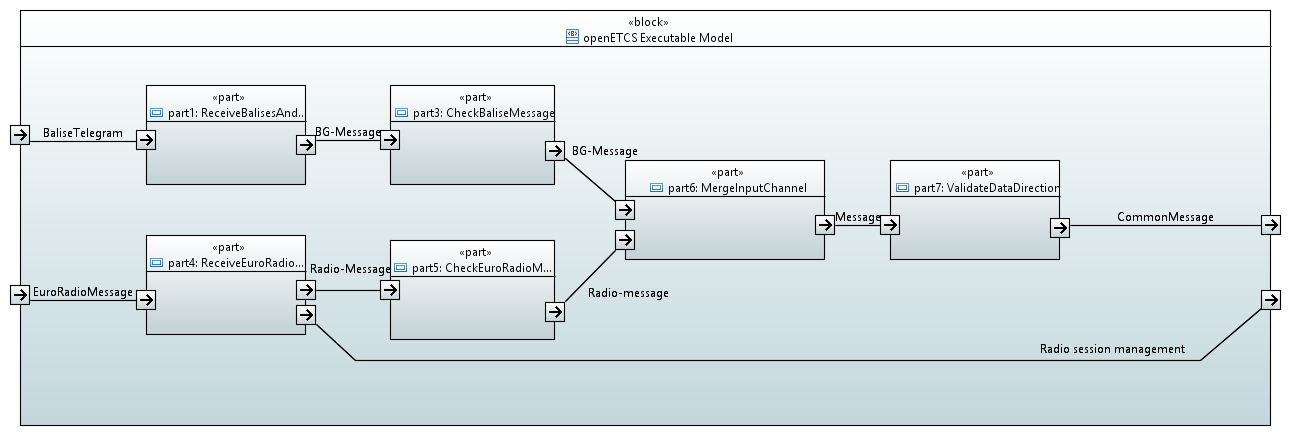
\includegraphics[width=\textwidth]{./images/Input-Messages4.PNG}
 % Input-Messages4.PNG: 0x0 pixel, 0dpi, nanxnan cm, bb=
 \caption{Structure of the Receive message and check consistency module}
 \label{fig:receiveAndCheckConsistencyArch}
\end{figure}
 
\subsubsection{Input}
For providing the output, the module needs different input data flows. An overview is provided in table \ref{tbl:ReceiveMessageAndCheckConsistencyInput}

\begin{table}[H]
  \begin{tabular}{| c | l | l | l | l |}
    \hline
    \textbf{Index} & \textbf{Input name} & \textbf{Input type} & \textbf{Source}\\ \hline
    0 & \texttt{apiRtmMessage} & \texttt{< will be defined by API >} & API \\
    1 & \texttt{apiBaliseTelegram} & \texttt{API\_Telegram\_T} & API\\
    2 & \texttt{apiRadioDevice} & \texttt{int} & API\\
    3 & \texttt{connectionStatus} & \texttt{sessionStatus\_Type} & MoRC\\
    5 & \texttt{lastRelevantEventTimestamp} & \texttt{T\_internal\_Type} & MoRC or Database (?)\\
    6 & \texttt{tNvContact} & \texttt{T\_internal\_Type} & Database\\
    7 & \texttt{currentOdometry} & \texttt{odometry\_T} & Odometry\\
    8 & \texttt{lrbg} & \texttt{positionedBG\_T} & Database\\
    9 & \texttt{reset} & \texttt{bool} & internal\\
    \hline
  \end{tabular} 
  \caption{Overview over input}
  \label{tbl:ReceiveMessageAndCheckConsistencyInput}
\end{table}

\paragraph{Input 0: \texttt{apiRtmMessage}}

The Euroradio-/Eurobalise-message is originated from the openETCS-API. The API is described in the section \ref{chp_openETCS_API}.

In the current implementation, only messages with normal priority are used in the system. Emergency messages will not be processed.

%The type \texttt{RTM\_IN\_MESSAGE\_T}  is used for normal messages, which can contain connection confirmations, information about connection problems or data.
%\begin{table}[H]
%	\begin{tabular}{| c | l | l | l |}
%	 \hline
%	 \textbf{Index} & \textbf{Element name} & \textbf{Element type} & \textbf{Description}\\ \hline
%	 0 & RADIO\_DEVICE & ETCS\_ID\_T & Source interface of the message\\
%	 1 & REASON & RTM\_DIAGNOSTIC\_CODE\_T & Diagnostic code for connection problems\\
%	 2 & DATA & RTM\_MESSAGE\_T & Decoded message, CRC-checked\\
%	 \hline
%	\end{tabular}
%\end{table}

The input not only transfers the radio message but also information, if a message is present and if this message was decoded correctly and passed the lowlevel checks performed by the API.

The radio message itself consists of a header and a payload-part. The header part contains all variables of the message. The payload-part consists of all packets in the message.

\paragraph{Input 1: \texttt{apiBaliseTelegram}}

The telegram is build from 
\begin{itemize}
\item a present flag (bool)\\
Indicates the input decoded telegram parameter is “present”, i.e., the input has been updated by the API.
Only if the telegram is present the position information (incenterOfBalise) is to be used.\\
\item the decoded telegram including optional packets received from the balise.
\item the centerOfBalisePosition parameter. This parameter is used to give the position where the BTM has recognised the center of the balise telegram.
\end{itemize}

\paragraph{Input 2: \texttt{apiRadioDevice}}
The RTM-module can consist of multiple radio devices. When a handover between two RBCs is performed, messages can be received from both radio devices. The API provides information about the device, which received the message.

The values transmitted have to be defined by the API.

\paragraph{Input 3: \texttt{connectionStatus}}
The input \texttt{connectionStatus} will give information about the radio connection. This input is delivered by the session management module, not from the API. The information is needed to perform a timestamp check, which is depending on the connection state.

\begin{table}[H]
  \begin{tabular}{| l | p{9cm} |}
    \hline
    \textbf{Value} & \textbf{Interpretation}\\ \hline
    DISCONNECTED & The OBU is currently not connected to a RBC.\\
    CONNECTING & The OBU is currently connecting to the RBC. Received messages belong to the process of establishing a connection.\\
    CONNECTION\_ESTABLISHED &  The connection to RBC is established.\\
    \hline
  \end{tabular} 
  \caption{Possible values for the input \texttt{connectionStatus}}
  \label{tbl:connectionStatus}
\end{table}

% \paragraph{Input 4: \texttt{apiConsistencyError}}
% If the API detects a consistency error in the transmitted message, this error is reported to the model by the input \texttt{apiConsistencyError}.
% 
% Possible errors detectable by the API are:
% \begin{itemize}
%  \item CRC-error
%  \item Value range of variable exceeded
% \end{itemize}
% 
% 
% \begin{table}[H]
%   \begin{tabular}{| l | p{9cm} |}
%     \hline
%     \textbf{Value} & \textbf{Interpretation}\\ \hline
%     true & The API detected a consistency error.\\
%     false & No consistency error was detected by the API.\\
%     \hline
%   \end{tabular} 
%   \caption{Possible values for the input \texttt{apiConsistencyError}}
%   \label{tbl:apiConsistencyError}
% \end{table}

\paragraph{Input 5: \texttt{lastRelevantEventTimestamp}}

For monitoring the safe radio connection, it's necessary, that the time between two packets is less than the value of \texttt{T\_NVCONTACT}.

In situations like level-changes or announced radioholes, not the timestamp of the last message is relevant for comparison, but the timestamp of the last relevant event. This can be e.g. the timestamp of the level change or the timestamp of the timestamp of the moment, when the train was passing the end of the radiohole. 

For performing this check, the timestamp of the last relevant event is provided to the model as an \texttt{T\_internal\_Type}-type.

\paragraph{Input 6: \texttt{tNvContact}}

For monitoring the safe radio connection, the national value \texttt{T\_NVCONTACT} is needed as an input.

\paragraph{Input 7: \texttt{currentOdometry}}
Current information giving the odometry of the train. 

\paragraph{Input 8: \texttt{lrbg}}
The Last Relevant Balise Group. The information has been collected before by the train position function.

\paragraph{Input 9: \texttt{reset}}
To delete all data stored in the module (e.g. collected balise-telegrams, which do not yet form a complete message), a reset input can be used. If the input is set to \texttt{true}, all data kept in the module is deleted and no input is accepted.

\begin{table}[H]
  \begin{tabular}{| l | p{9cm} |}
    \hline
    \textbf{Value} & \textbf{Interpretation}\\ \hline
    true & All data kept in the module is deleted and no input is accepted.\\
    false & No action. Data at input is accepted.\\
    \hline
  \end{tabular} 
  \caption{Possible values for the input \texttt{reset}}
  \label{tbl:reset}
\end{table}

% A Eurobalise telegram consists of several fields shown in the table below. The table is an excerpt from the SRS, chapter 8.4.2.1. In this chapter the description of the fields can be found.
%  
%  
%  \begin{tabular}{| c | l | c  |}
%   \hline
%   \textbf{Field No.} & \textbf{VARIABLE} & \textbf{Length (bits)} \\ \hline
%   1 & Q\_UPDOWN & 1\\
%   2 & M\_VERSION & 7\\
%   3 & Q\_MEDIA & 1\\
%   4 & N\_PIG & 3\\
%   5 & N\_TOTAL & 3\\
%   6 & M\_DUP & 2\\
%   7 & M\_MCOUNT & 8\\
%   8 & NID\_C & 10\\
%   9 & NID\_BG & 14\\
%   10 & Q\_LINK & 1\\
%   \textit{-} & \textit{Packet 0 (Virtual balise cover) (optional)} & \textit{14}\\
%   \textit{-} & Information & variable\\
%   \textit{-} & Packet 255 & 8\\  
%   \hline
%  \end{tabular}
%  
%  \textbf{Relevant messages for track Utrecht-Amsterdam:} packets from balises: 3, 41, 42, 45, 46, 65, 72, 137, 255
%  
 


% \begin{itemize}
%  \item packets from balises: 3, 41, 42, 45, 46, 65, 72, 137, 255
% \end{itemize}
% \item unchecked Euroradio message
% \begin{itemize}
%  \item messages from rbc: 2, 3, 6, 8, 15, 24, 27, 32, 39, 41
%  \item packets from rbc: 3, 5, 15, 21, 27, 41, 42, 57, 58, 65, 68, 72, 80
% \end{itemize}
%\end{itemize}


\subsubsection{Output}
The output of the module provides the received and processed Euroradio and Eurobalise messages. The module combines messages both from Eurobalises and from Euroradio to one common dataflow.

Additionally, status information is provided. The status information consists of the following data:
\begin{itemize}
	\item Information, if the message has to be rejected in case of a consistency error, includeing further information about the error.
	\item Information, if an acknowledgement has to be sent to the RBC for the message
	\item Information about the radio connection. None or one of the following notifications:
	\begin{itemize}
		\item Confirmation for establishing a connection or reconnection
		\item Notification, that a established connection was lost, including the origin of the failure
		\item Notification, that a connection could not be (re)established after 3 attempts, includeing the origin of the failure
		\item Notification, that a connection could not be re-established after 3 attempts, includeing the origin of the failure
	\end{itemize}
\end{itemize}

An overview over the output dataflows is provided in table \ref{tbl:ReceiveMessageAndCheckConsistencyOutput}.

\begin{table}[H]
  \begin{tabular}{| c | l | l | l |}
    \hline
    \textbf{Index} & \textbf{Output name} & \textbf{Output type}\\ \hline
    0 & \texttt{present} & \texttt{bool}\\
    1 & \texttt{rejectionReason} & Boolean-Array (to be defined)\\
    2 & \texttt{acknowledgementRequired} & \texttt{bool}\\
    3 & \texttt{radioConnectionStatusFromAPI} & \texttt{RadioConnectionStatusFromAPI\_T}\\
    4 & \texttt{radioDeviceOut} & \texttt{int}\\
    5 & \texttt{applyServiceBreak} & \texttt{bool} \\
    6 & \texttt{badBaliseMessageToDMI} & \texttt{bool} \\
    7 & \texttt{receivedMessage} & \texttt{ReceivedMessage\_T} \\
    \hline
  \end{tabular} 
  \caption{Dataflow at output}
  \label{tbl:ReceiveMessageAndCheckConsistencyOutput}
\end{table}

\subparagraph{Output 0: \texttt{present}}
The present-flag specifies, if the data provided by the output \texttt{receivedMessage} is to be considered as present by the following modules or if it has to be ignored due to no new input data.

\begin{table}[H]
  \begin{tabular}{| l | p{13cm} |}
    \hline
    \textbf{Value} & \textbf{Interpretation}\\ \hline
    false & The data in this element is not present and has to be ignored. \\
    true & The data in this element is present and has to be processed by the following models. \\
    \hline
  \end{tabular} 
  \caption{Possible values for the output \texttt{present}}
  \label{tbl:rcvpresent}
\end{table}

\subparagraph{Output 1: \texttt{rejectedReason}}
In case of an inconsistent message, the output \texttt{rejectedReason} is giving information to the system, which problem occured. This information also has to be sent to the RBC as an error report.

\subparagraph{Output 2: \texttt{acknowledgementRequired}}

The \texttt{acknowledgementRequired}-dataflow indicates, whether the reception of the message has to be acknowledged to the RBC.

\begin{table}[H]
  \begin{tabular}{| l | p{13cm} |}
    \hline
    \textbf{Value} & \textbf{Interpretation}\\ \hline
    true & An acknowledgement has to be sent to the RBC for the current message delivered at output \texttt{receivedMessage} \\
    false & No acknowledgement has to be sent for the current message delivered at output \texttt{receivedMessage} \\
    \hline
  \end{tabular} 
  \caption{Possible values for the output \texttt{AcknowledgementRequired}}
  \label{tbl:AcknowledgementRequiredTable}
\end{table}

\subparagraph{Output 3: \texttt{radioConnectionStatusFromAPI}}
The output \texttt{radioConnectionStatusFromAPI} is used, when the RTM reports problems with the radio connection. The output is derived from the Alstom-API. %\textbf{TODO!} 
The output can be one of the following values:

\begin{table}[H]
  \begin{tabular}{| l | p{9cm} |}
    \hline
    \textbf{Value} & \textbf{Interpretation}\\ \hline
    CONNECTION\_CONFIRMATION & Confirmation for establishing a connection or reconnection\\
    CONNECTION\_LOST & Notification, that a established connection was lost\\
    CONNECTION\_FAILURE & Notification, that a connection could not be (re-)established after 3 attempts, includeing the origin of the failure\\
    
    CONNECTION\_NOT\_ESTABLISHED &  Notification, that a connection could not be re-established after 3 attempts, includeing the origin of the failure\\
    \hline
  \end{tabular} 
  \caption{Possible values for the output \texttt{radioConnectionStatusFromAPI}}
  \label{tbl:ConnectionStatusOutput}
\end{table}

\subparagraph{Output 4: \texttt{radioDeviceOut}}
The output radio device will give information, which device received a radio message. Trains equipped with two or more radio devices may receive messages on two interfaces in situations of a RBC handover.

\subparagraph{Output 5: \texttt{applyServiceBreak}}
The flag indicates the balise group the train just passed could not be processed correctly. The check results in the request for a service break.

\subparagraph{Output 6: \texttt{badBaliseMessageToDMI}}
Information to be passed to the DMI to indicate the reception of a ``bad balise'' to the driver.

\subparagraph{Output 7: \texttt{receivedMessage}}
The element \texttt{receivedMessage} consists of the type \texttt{ReceivedMessage\_T} combines both balise and radio messages to one common datatype. This datatype contains all variables and packets, which are possible for the given scenario.

\begin{table}[H]
  \begin{tabular}{| l | l | p{5.5cm} |}
  \hline
  \textbf{Name} & \textbf{Datatype} & \textbf{Description}\\ \hline
  source & Enumeration & Defines, if this is a Euroradio or Eurobalise message.\\
  valid & bool & true, if no consistency errors were detected.\\
  BG\_Common\_Header & \texttt{BG\_Header\_T} & Header of Eurobalise message\\
  Radio\_Common\_Header & \texttt{Radio\_TrackTrain\_Header\_T} & Header of Euroradio message\\
  Packets & structure of possible packets & -\\
  
  \hline
\end{tabular}
  \caption{Structure of \texttt{ReceivedMessage\_T}}
  \label{tbl:receivedMessage_structure}
\end{table}

The Eurobalise-common-header \texttt{BG\_Header\_T} consists of the fields visible in the SCADE-declaration. The structure corresponds to the structure defined in the SRS chapter 8.4.2.1. Some fields were removed since they are not needed anymore for further processing after building messages from separate telegrams.

The Euroradio-common-header \texttt{Radio\_TrackTrain\_Header\_T} consists of the fields visible in the SCADE declaration. The structure corresponds to the structure defined in the SRS chapter 8.4.4.6.1. The structure contains all variables required by possible \texttt{NID\_MESSAGE} values for the given scenario.

%\textbf{TODO:} Different definition of Radio-header than in SCADE!

%\textbf{TODO:} Note on packet type definitions and implementation details (which values were not used).

\textbf{Note:} Packet 44 not used (applications outside the ERTMS/ETCS system are not supported by this implementation).

%\textbf{TODO:} Define packets 136, 12 in SCADE.

\subsubsection{Data}
The function makes use of internal data for collecting and checking the balise telegrams.

\subsubsection{Reference to the SRS (or other requirements)}
\paragraph{Eurobalise}
\begin{itemize}
  \item Definition of the Balise Telegram: subset 26 section 7 and 8
  \item Interface to the BTM: Subset 36, section  4.2.2, 4.2.4, 4.2.9
  \item Handling of Balise Telegrams: Subset 26, sections 3.4.1 - 3.4.3, 3.16.2
  \item Check of the balise group Subset 26, section 3.16.2
  \item Determining the Orientation: 3.4.2
  \item Active Functions Table: 4.5.2
\end{itemize}

\paragraph{Euroradio}
\begin{itemize}
 \item SRS subset 26, chapter 8.4.4: Rules for Euroradio messages
 \item SRS subset 26, chapter 3.16: Data consistency
\end{itemize}

\paragraph{ValidateDataDirection}
\begin{itemize}
 \item The functionality is mainly described in \cite[Chapter~3.6.3]{subset-026}.
\end{itemize}

\subsubsection{Design Constraints and Choices of submodules}

\paragraph{Reception of messages}

The first stage of the module is the reception of Euroradio-messages and Eurobalise-Telegrams from the openETCS-API. At each cycle the following conditions can occur:
\begin{enumerate}
 \item No new Euroradio-message or Eurobalise-telegram is available.
 \item A new Euroradio-message is available
 \item A new Eurobalise-telegram is available
 \item A new Euroradio-message and a new Eurobalise-telegram is available.
\end{enumerate}

\paragraph{Part 1: ReceiveBaliseAndBuildBG}\label{ss:ReceiveEurobaliseFromAPI}

This function defines the interface of the OBU model to the openETCS generic API for Eurobalise Messages. On the interface, either a valid telegram is provided or a telegram is indicated which could not be received correct when passing the balise. The function passes the telegram without major changes of the information to the next entity for collecting the balise group information. This entity collects telegrams received via the interface into Balise Group Information.
	
\textbf{Design Constraints and Choices}
\begin{enumerate}
\item The decoding of balises is done at the API. Also, packets received via the interface are already transformed into a usable shape.
\item Only packets used inside the current model are passed via the interface:\\
Packet 5: Linking Information.\\
Linking Information is added to the linking array starting from index 0 without gaps. Used elements are marked as valid. Elements are sorted according to the order given by the telegram sequence.
\item Telegrams received as invalid are passed to the ``Check-Function'' to process errors in communication with the track side according to the requirements and in a single place.
Telegrams are added to the telegram array starting from index 0 without gaps. Used elements are marked as valid. Elements are stored according to the order given by the telegram sequence.
\item This function does not process information from the packets. The information is passed to the check without further processing of the values. 
\end{enumerate}

\paragraph{Part 3: Check BG Consistency}

\subparagraph{Short Description of Functionality}
This function has the task  to verify the completeness and correctness of the received messages from balis-groups.\\
A message consists of at least a telegram and a maximum of 8 telegrams.\\

\begin{itemize}
\item A message is still complete and correct, if a telegram is missing (or not decoded or incomplete decoded ), and this telegram is duplicated within the balise group and the duplicating one is correctly read.
\item By more than one telegram, the order of the telegrams must be either ascending (nominal ) or Descending(reverse).\\
\item A message is correct, if  all message counters (M MCUNT) do not equal 254 (that means: The telegram never fits any message of the group).\\ A message counter can be equal 255 (that means: The telegram fits with all telegrams of the same balise group) and all other values must be the same.\\
\end{itemize}

\subparagraph{Design Constraints and Choices}

%\begin{enumerate}
%\item Only packets used inside the current model are passed via the interface:\\
%Packet 5: Linking Information.\\
%\item In this function packets past with the telegrams is accumulated into a balise group information.\\
%\item Further assumption on packet 5 (based on SRS subset 26, section 8.4.1.4)\\
%(In this statement the term ``message'' is ambiguous since it can reflect to a telegram or a balise group message)
%Linking Information can only be passed once. This means, if linking information for the balise group is already collected with one of the earlier telegrams, the information will not be accumulated but overwritten.\\
%\end{enumerate}
This function is active in certain modes and the output and reactions are dependent on if the linking information is used.\\
The orientation of the BG will also be calculated in this block.\
The check, if the message has been received in due time and the right at the right expected location, will be performed in "Calculate Train Position".\\
The checks on the validity of the data in the packets and the validity with respect to the direction of motion will be performed in other modules, e.g. "Validate Data Direction" .

%\paragraph{Validate direction}
%\begin{itemize}
%	\item Identify direction validity of message (SRS 3.6.3.1.2)
%	\item If the message is not desired for the direction of train movement, the message shall be \textbf{ignored}. (SRS 3.6.3.1.3)
%	\item If the train position is unknown, only data valid for both directions shall be accepted. Other data shall be \textbf{rejected}. (SRS 3.6.3.1.3.1)
%	\item If a single balise group requires the knowledge of an coordinate system, but no coordinate system was  assigned, data valid only for one direction shall be \textbf{rejected}. Exception: Data for National Systems. (SRS 3.6.3.1.4 / 3.6.3.1.4.1)
%	\item The implementation has to take care of exceptions 
%\end{itemize}






% \subsection{F.1.5 Select Usable Info - Mode and Level Filter}
% 
% \paragraph{Short Description of Functionality}
% The function Select Usable Info filters information received from balises that have been passed, radio messages, and EUROLOOP messages. Filtering is done depending on the mode of the train, the current ETCS level, the type/content of the information, and the transition media of the information. As neither radio messages nor EUROLOOP are part of the first iteration of work, not all functionality of the filter described in the specification is currently implemented.
% 
% \paragraph{Reference to the SRS (or other requirements)}
% The functionality of Select Usable Info is described in Chapter 4.8 of subset-026 \cite{subset-026}. The following list gives an overview of the most important sections for each of the blocks in the model.
% 
% \begin{description}
% \item[First filter] The first filter, i.e.~the filter on the level, is described in \cite[Chapter~4.8.3]{subset-026}.
% \item[Second filter] The second filter, i.e.~the filter on the transition media, is described in\cite[Chapter~4.8.3]{subset-026}.
% \item[Third filter]
%  The third filter, i.e.~the filter on the modes, is described in \cite[Chapter~4.8.4]{subset-026}.
% \item[Transition buffers] Details on the handling of the transition buffers used in the first and the second filter are described in \cite[Chapter~4.8.5]{subset-026}.
% \end{description}
% 
% \paragraph{Design Constraints and Choices}
% The first iteration of the model takes only balise group messages into account. This implies that a large part of the specification of this function described in subset-026 \cite{subset-026} is not relevant for the first iteration. This in particular applies to the second filter, i.e.~filter on the transition media, because radio messages are not part of the model so far. Moreover, the functionality of the first filter, i.e.~filter on the level, is currently  limited because the first iteration of the model implements ETCS level 1 only.
% 
% \paragraph{Filtering (Mode/Level) - One packet per type}
% \textbf{ISSUE: HOW MANY PKT 44, 65 AND 66 PER MESSAGE ARE MAXIMALLY SUPPORTED? (BH: who made this comment??)}\\
% 
% - Check on announced and immediate level transition orders in the messages to be filtered (needed for further criteria for filtering, to decide if the data shall be stored in the transition buffer).\\
% - Filter data stored in the transition buffer according to the current level (what to do if similar information is available in the new message??). Data can be rejected, accepted or kept in the transition buffer.
% (Filtering according to new level will be done directly afterwards in the next cycle)\\
% - Filter new received messages according to the current level (new level will be done in the next cycle as according to \gls{SRS} data first has to be filtered according to old level and afterwards to new level). Data can be rejected, accepted or stored in the transition buffer.\\
% - Filter (level) accepted data according to originating RBC (supervising or other). Information from \gls{BG}'s, loops or RIU is not filtered with this filter.\\
% - Filter (level and RBC) accepted data according to the current mode (only reject or accept)\\

\paragraph{Part 5: CheckEuroradioMessage}
``CheckEuroradioMessage'' has to perform several checks on the received radio message.

\begin{itemize}
 \item Content checks
 \begin{itemize}
    %\item The computed length of the message must be equal to the value in \texttt{L\_MESSAGE}. (SRS 8.4.4.2.1)
    \item The whole message must be complete and contains all necessary fields. (SRS 8.16.1.1)
    \item The message must respect the ETCS language. (SRS 8.16.1.1)
    \item The variables of the message does not contain invalid values. (SRS 8.16.1.1) % already done by API?
    \item Check if the specified priority of message is equal to the priority with which the message was received. (SRS 3.16.3.1.3.1) 
  \end{itemize}
  \item Timing checks
  \begin{itemize}
    \item Check if the timestamp of a message is greater than the timestamp of the former message (SRS 3.16.3.3.3)
    \item If a message contains the timestamp ``Unknown'', check if this message is part of the initiation of the communication session. (SRS 3.16.3.3.4)
    \item Perform the check with the current packet $n$:  $T\_TRAIN_{n} <= T\_TRAIN_{n-1} + T\_NVCONTACT$ (SRS 3.16.1.1). This ensures, that the packet was received in due time.
  \end{itemize}
\end{itemize}

For inconsistent messages, the following actions need to be performed by the module:

\begin{itemize}
  \item If a message is not consistent, it shall be rejected (SRS 3.16.3.1.1.1). For this purpose, the message is marked as invalid.
  \item The RBC shall be informed, when a message was rejected (SRS 3.16.3.1.1.2). Therefore the message is marked with necessary information for creating an error report. 
  \item If the RBC requested an ACK for a received message, message will be marked for the module to send a report to the RBC. (SRS 3.16.3.5)
  \item This module will not trigger the reaction for an interrupted radio connection to the RBC. The reaction sepcified by \texttt{M\_NVCONTACT} will be triggered by the RBC session management module.
\end{itemize}

The check by the Euroradio-protocol (3.16.3.1.1) will not be performed by the model, but on a lower level (RTM or openETCS-API).

Safe connection supervision is not in the scope of this module. This functionality will be implemented by the ``Manage Radio communication'' module. The ``Receive message and check consistency''-module will provide the necessary status data about the connection as an output.

\subsubsection{Part 7: ValidateDataDirection}

\paragraph{Short Description of Functionality}
This function determines for direction information of the LRBG or an (ordinary) balise group whether this information is valid or not. The function takes as an input the LRBG and the balise groups passed and outputs the input extended with validity information.

\paragraph{Reference to the SRS (or other requirements}


\paragraph{Design Constraints and Choices}
none

\subsection{F.1.5 Select Usable Info - Mode and Level Filter}

\paragraph{Short Description of Functionality}
The function Select Usable Info filters information received from balises that have been passed, radio messages, and EUROLOOP messages. Filtering is done depending on the mode of the train, the current ETCS level, the type/content of the information, and the transition media of the information. As neither radio messages nor EUROLOOP are part of the first iteration of work, not all functionality of the filter described in the specification is currently implemented.

\paragraph{Reference to the SRS (or other requirements)}
The functionality of Select Usable Info is described in Chapter 4.8 of subset-026 \cite{subset-026}. The following list gives an overview of the most important sections for each of the blocks in the model.

\subsubsection{Interfaces}

\textbf{Input from:} Receive MSG Check Consistency/Coordinate System - track messages and package\\
Level and Mode Management - Mode and Level State\\

\textbf{Output to:} Build Data structure and Location Based/ Build Data Structures Drivers- forwarded packages, messages and variables\\

\begin{figure}[hbtp]
\centering
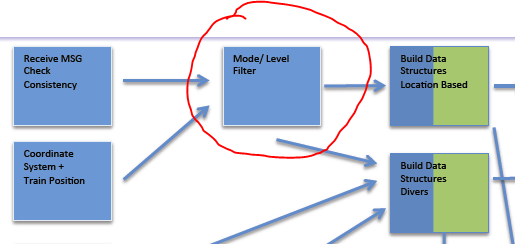
\includegraphics[scale=0.7]{images/FilterInandOUt}
\caption{Filter In and out}
\end{figure}

\subsubsection{SysML Model}
\begin{figure}[hbtp]
\centering
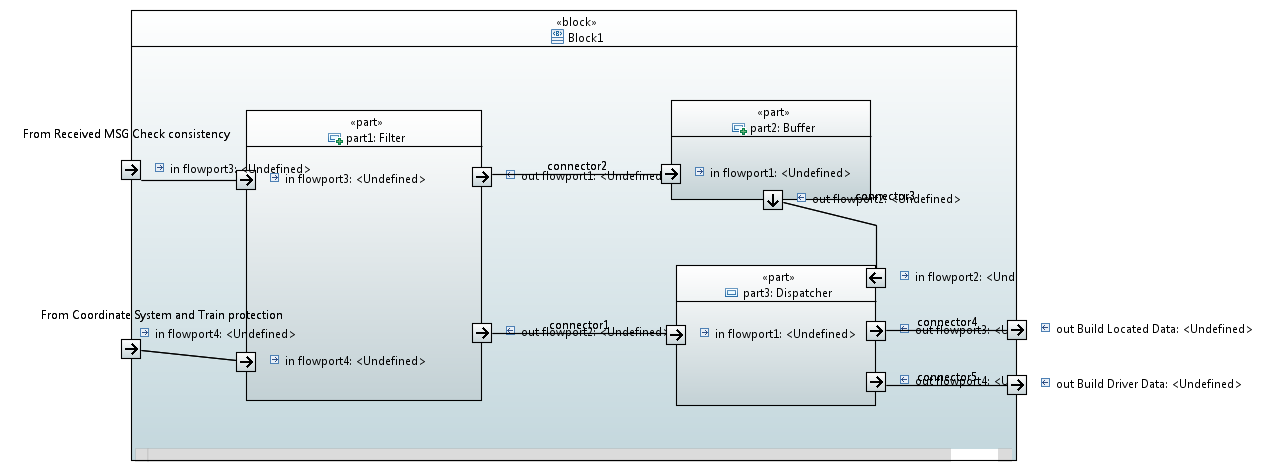
\includegraphics [scale=0.5]{images/SysMLFilter}
\caption{SysML Filter}
\end{figure}


\paragraph{Design Constraints and Choices}
The fillter receives track information (balise an radio) and will filter them in dependency of the mode and level.
Therefore the filter needs the input from level and mode management. The filtered information will be forwarded to the data strcuture.

\begin{description}
\item[First filter] The first filter, i.e.~the filter on the level, is described in \cite[Chapter~4.8.3]{subset-026}.
\item[Second filter] The second filter, i.e.~the filter on the transition media, is described in\cite[Chapter~4.8.3]{subset-026}.
\item[Third filter]
 The third filter, i.e.~the filter on the modes, is described in \cite[Chapter~4.8.4]{subset-026}.
\item[Transition buffers] Details on the handling of the transition buffers used in the first and the second filter are described in \cite[Chapter~4.8.5]{subset-026}.
\end{description}


\paragraph{Rererence to SRS: § 4.8.2, § 4.8.2, § 4.8.3, § 4.8.4}

\paragraph{Documentation of design}
From § 4.8.1.2 The following sections have to be interpreted by applying the filters and the assigned packets/messages as shown in Figure a and 2. The first filter is detailed in section § 4.8.3 (figure 1) “Accepted information depending on the level and transmission media”, the third filter in section § 4.8.4 (figure 2) “Accepted information depending on the modes”.\\

From § 4.8.1.3 If a message contains level transition information, any other information in that message shall be evaluated considering the level transition information. Explanation: If a message contains level transition information, all other information in that message shall be buffered and level transition shall be read first. Then the remained balise information shall be read from the buffer in the level that was announced to the balise.\\

From § 4.8.1.3.1 Information received in the same message as an immediate level transition order or a conditional level transition order that causes a level transition shall be evaluated first considering the on-board currently operated level, as if a level transition order for further location had been received (i.e. conditions [1], [2] or [6] of Figure 1, if applied, shall be automatically fulfilled). Then, if relevant, it shall be immediately extracted from the buffer and re-evaluated according to the new selected level.\\
\textbf{Explanation:} As described in Explanation of § 4.8.1.3 and figure 1 – First Filter conditions [1], [2] and [6])\\

From § 4.8.1.4 Note: As shown in Figure 1, information stored following an announcement of a change of level, is re-checked for acceptance when the level has changed. This implies that, when the level changes, the mode is - for a short moment – still unchanged, until the stored information has been processed. The consequence for the Third Filter is that information needs to be accepted for this short period also in modes in which this information is otherwise useless.\\
\textbf{Explanation:} when a level announced the level the mode change will be unchanged until the buffered information has been processed. The model change is the third filter (§ 4.8.3 figure 3).\\

\paragraph{table for the filter rules}
\textbf{Assumptions from § 4.8.2 need to be considered}\\
\textbf{Explanation}: See figure 1 and 2 – announced packets/messages/variables to the filter. Exception and explanation of the meaning of R and A please read § 4.8.3.\\. 

\textbf {Filter rules}: Filter will filter messages, packages and variables. Therefole a rule must be defined to cover all these inputs.\\

\textbf {Explanation figure 1}: will filtering the different inputs in dependency of the level\\
\textbf {Explanation figure 2}: will filtering the different inputs in dependency of thel mode\\

\paragraph{Filter on Level}
\begin{figure}[hbtp]
\centering
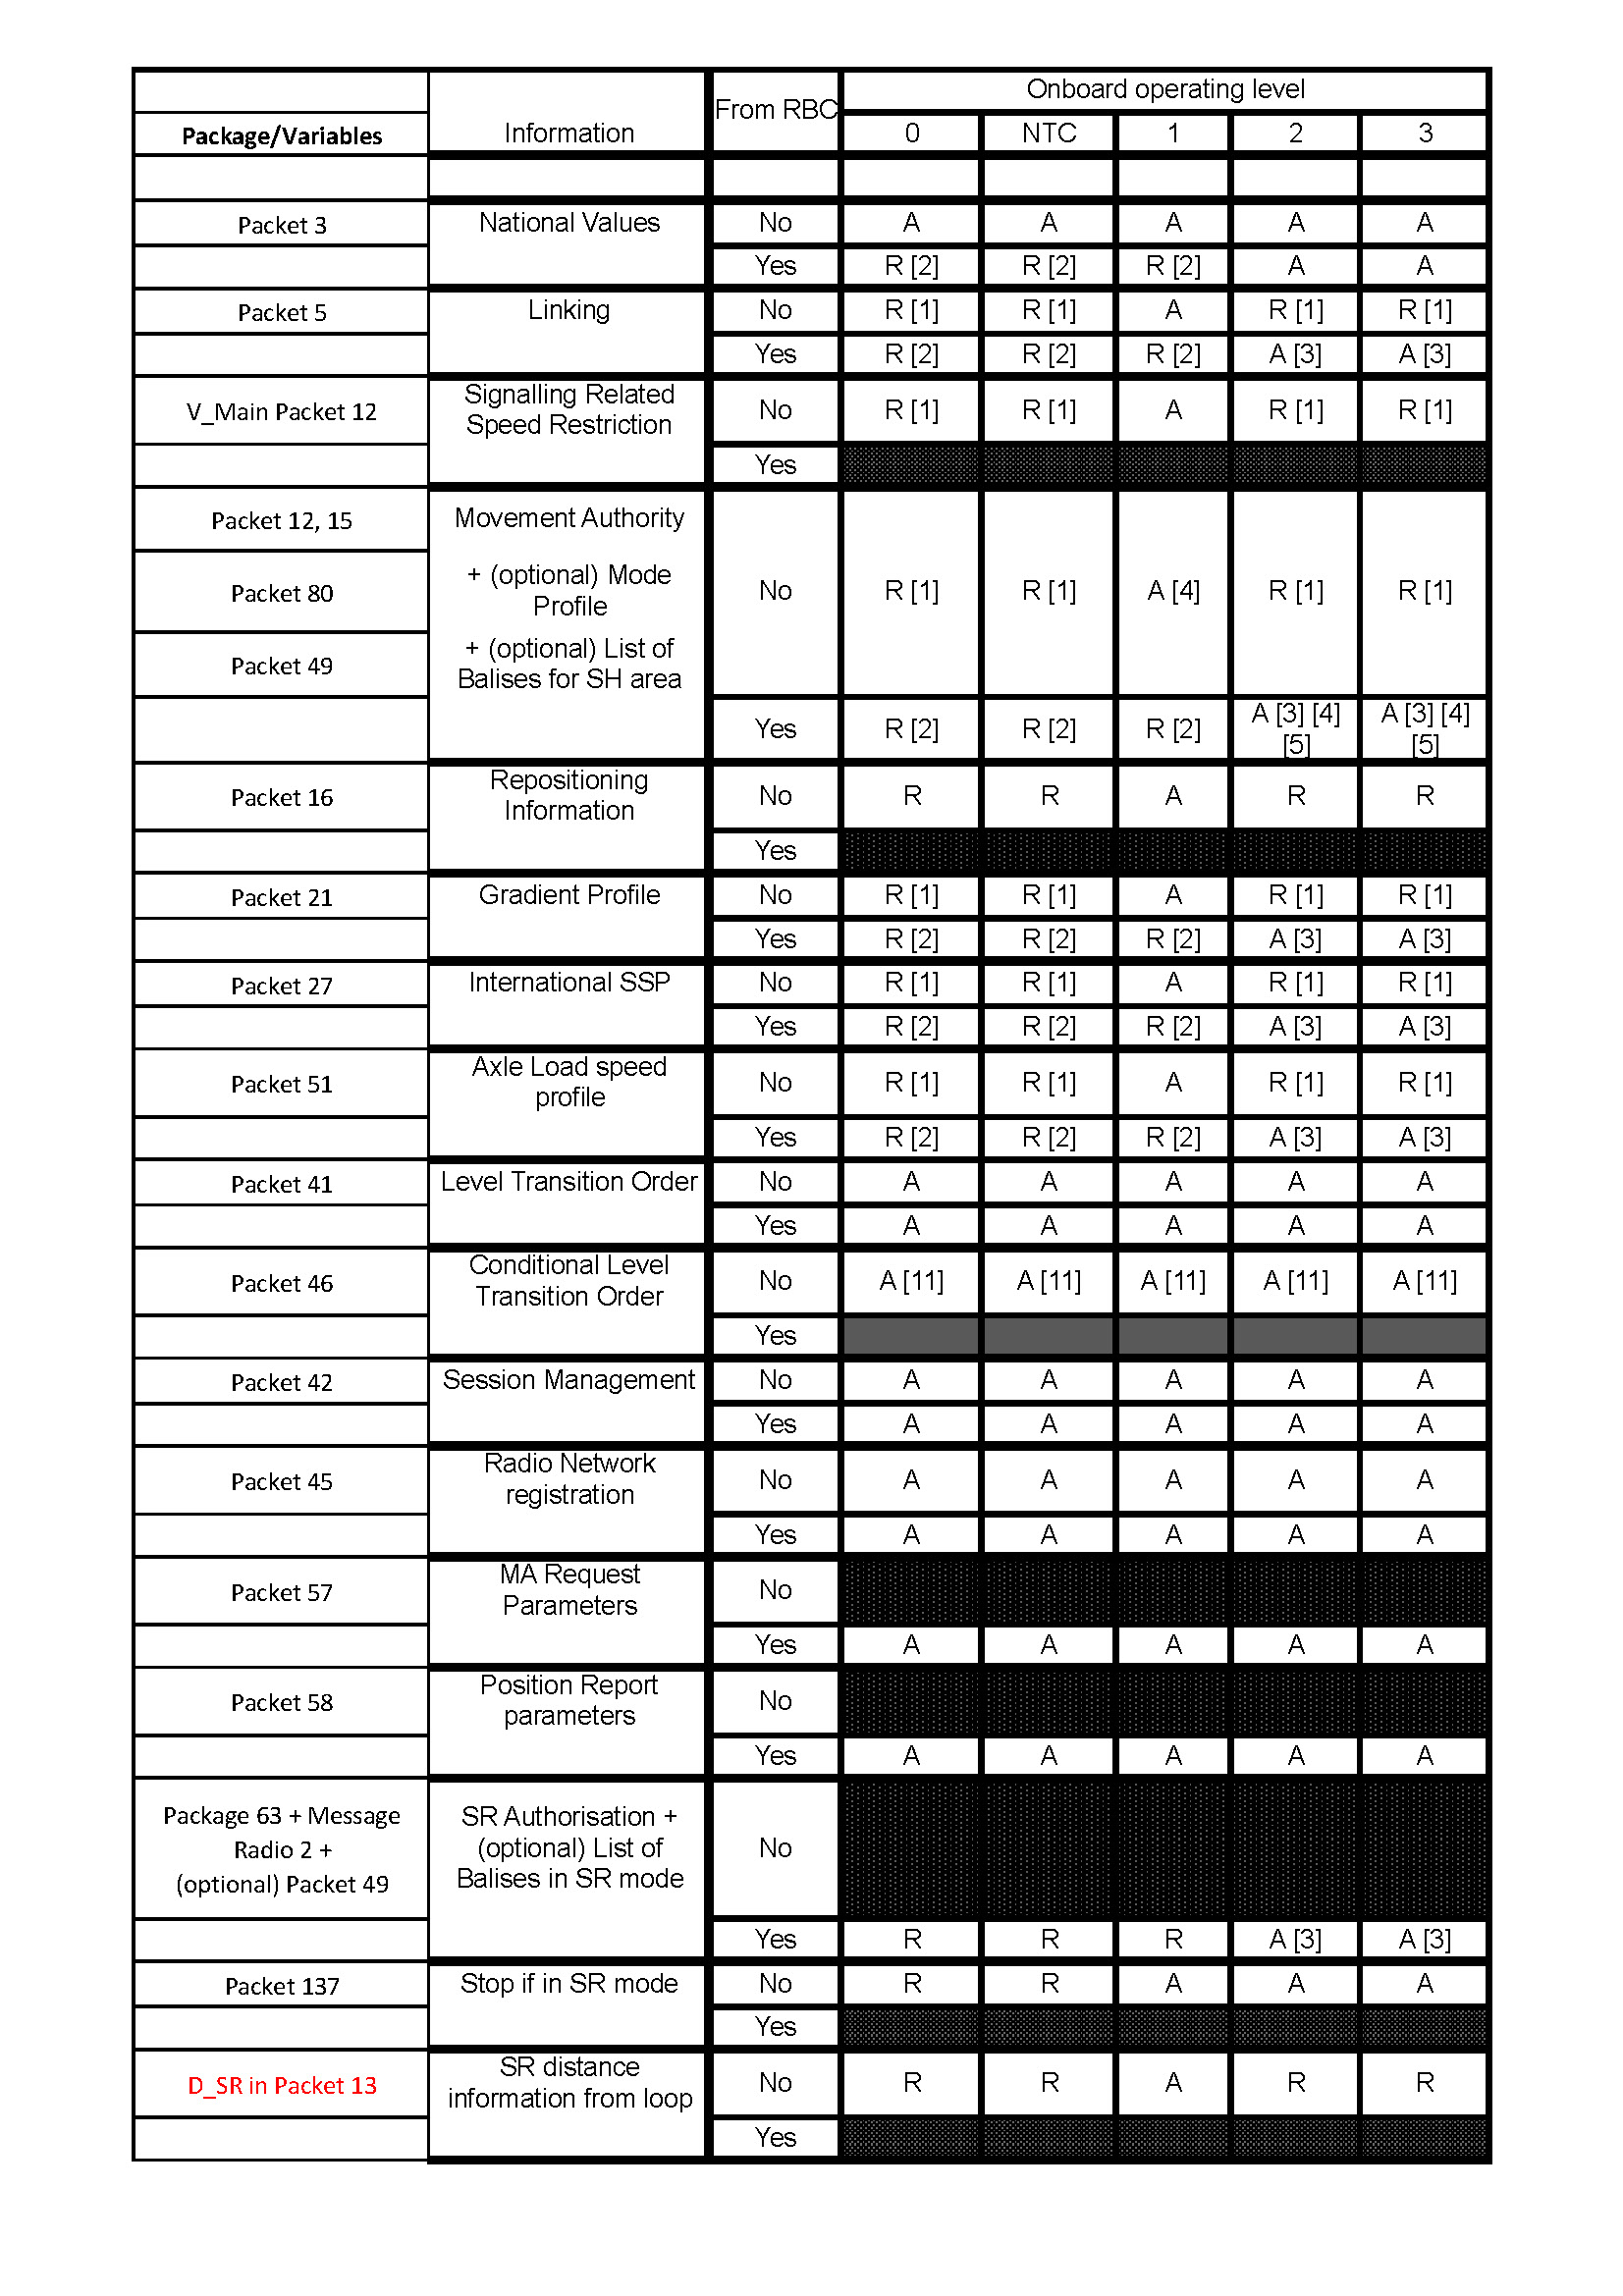
\includegraphics [scale=0.6]{images/LevelFilter1}
\end{figure}
\begin{figure}[hbtp]
\centering
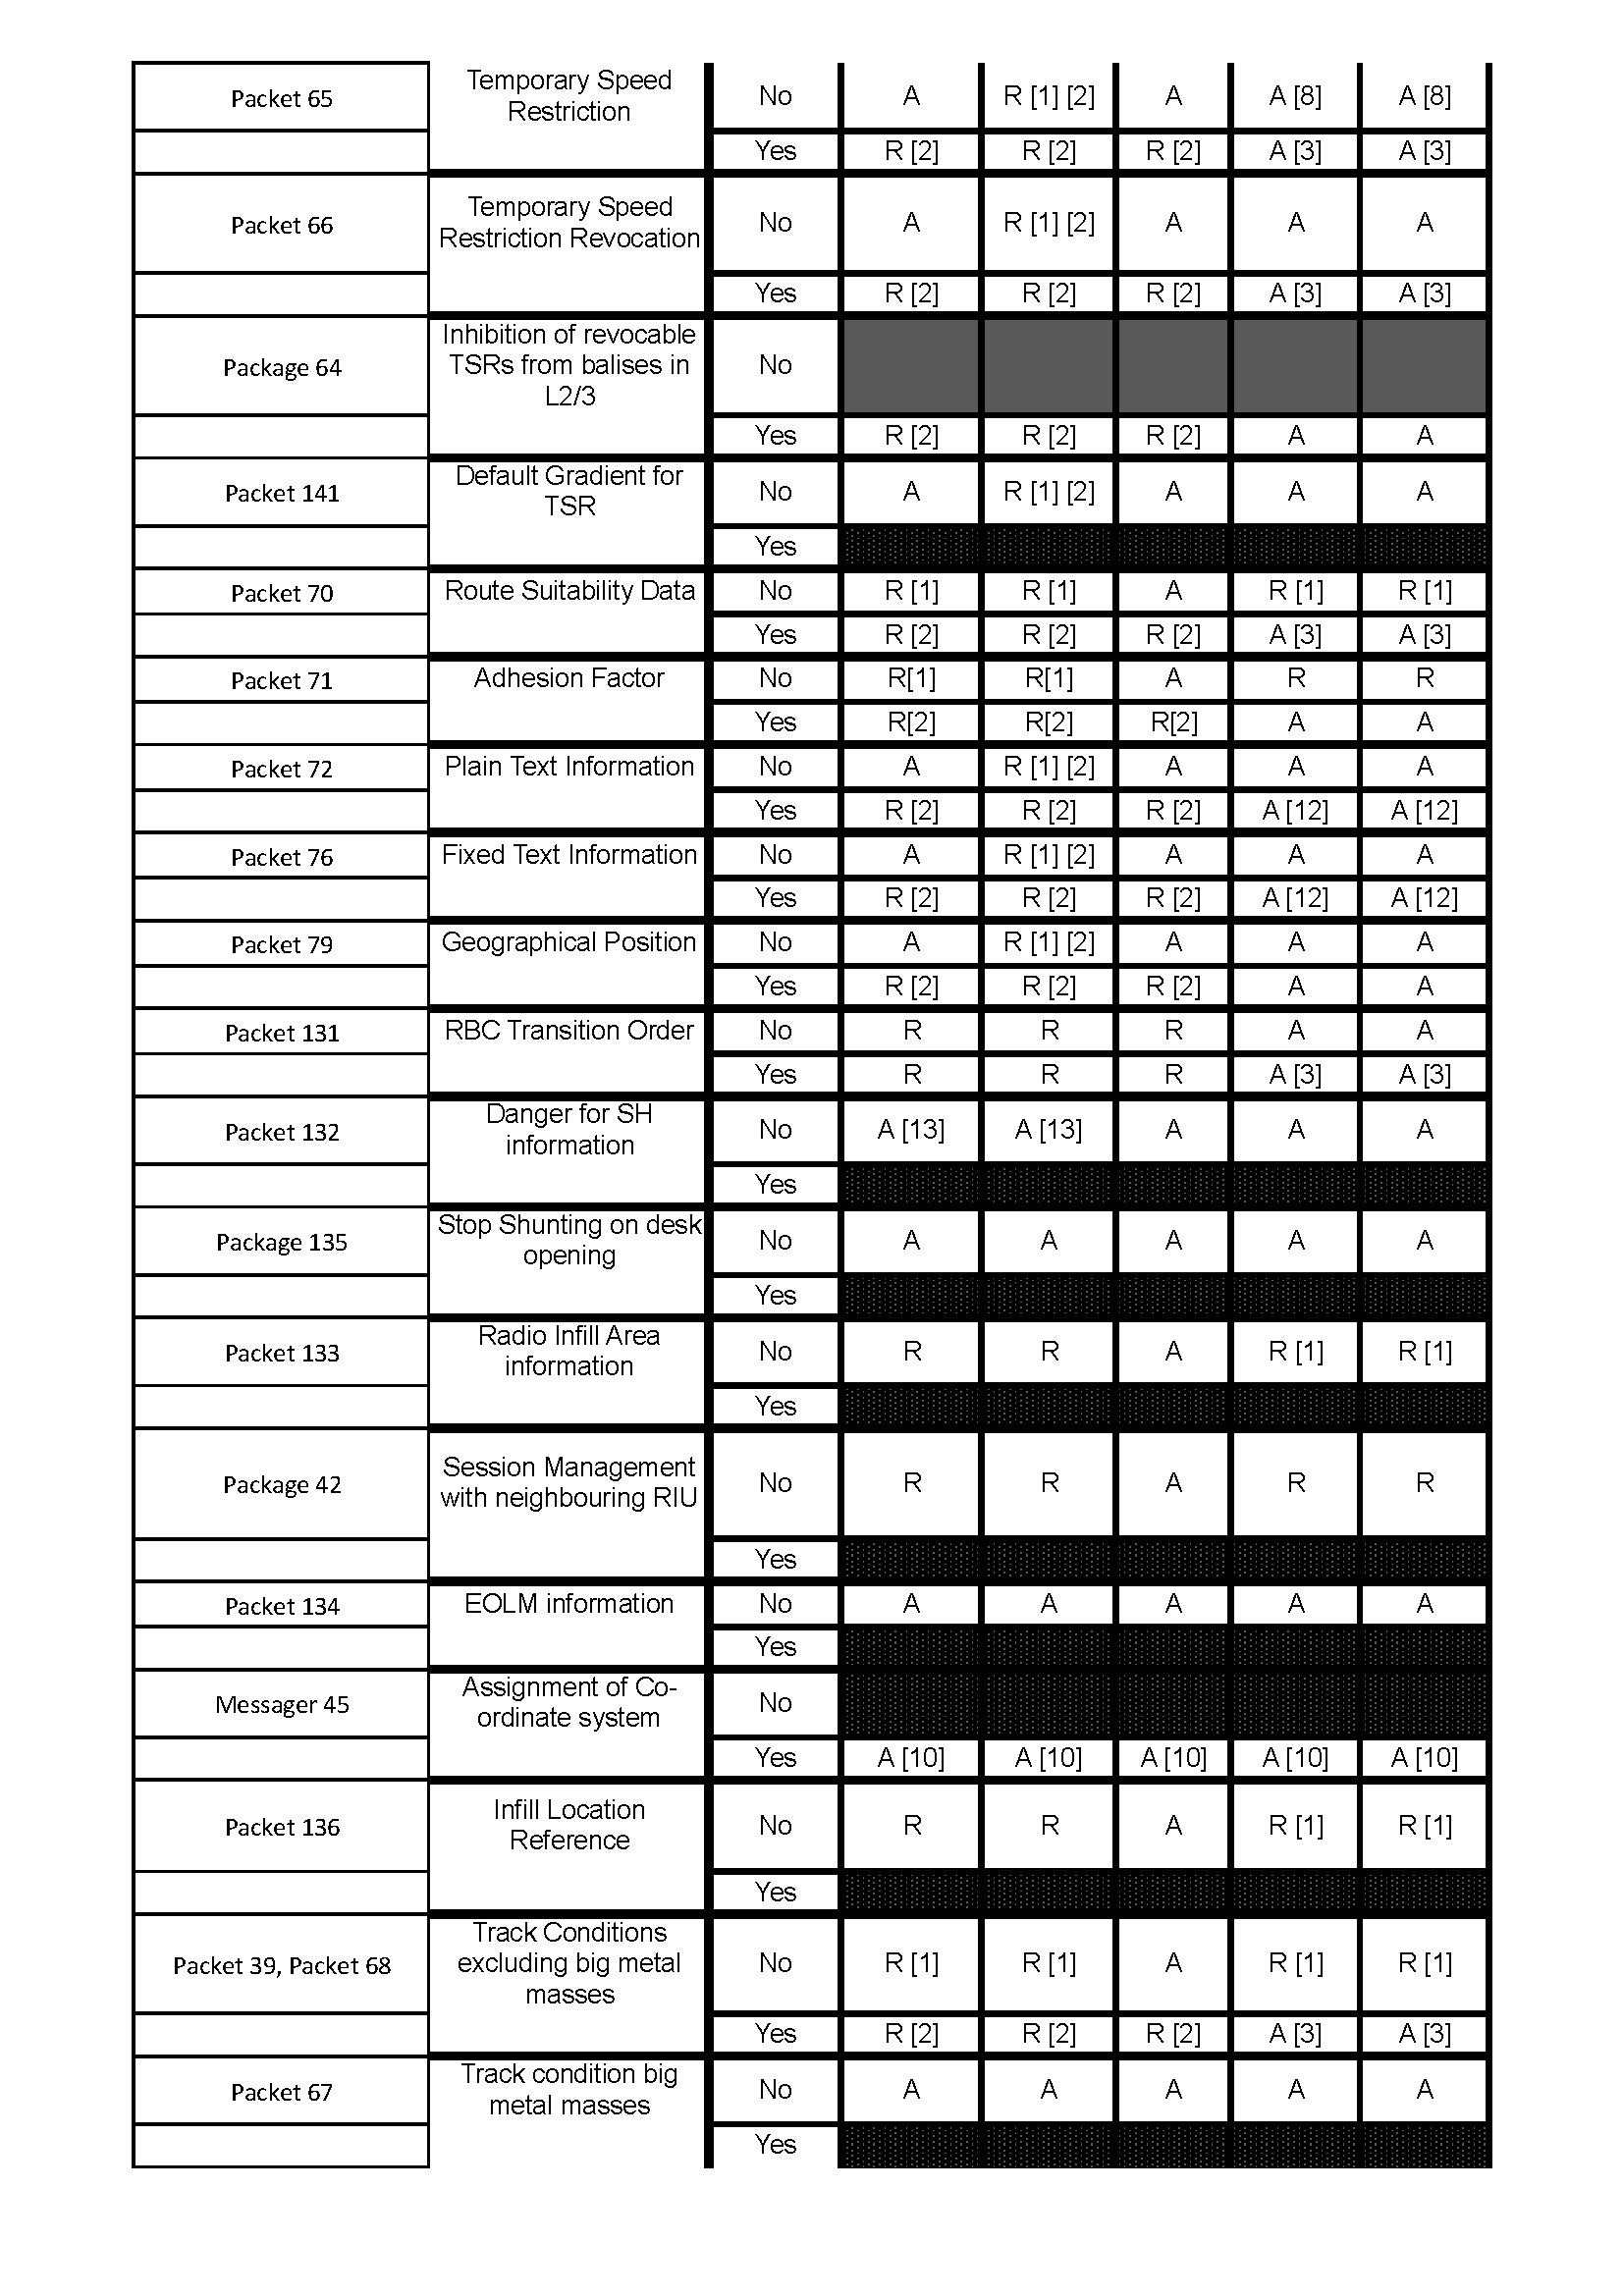
\includegraphics [scale=0.6]{images/LevelFilter2}
\end{figure}
\begin{figure}[hbtp]
\centering
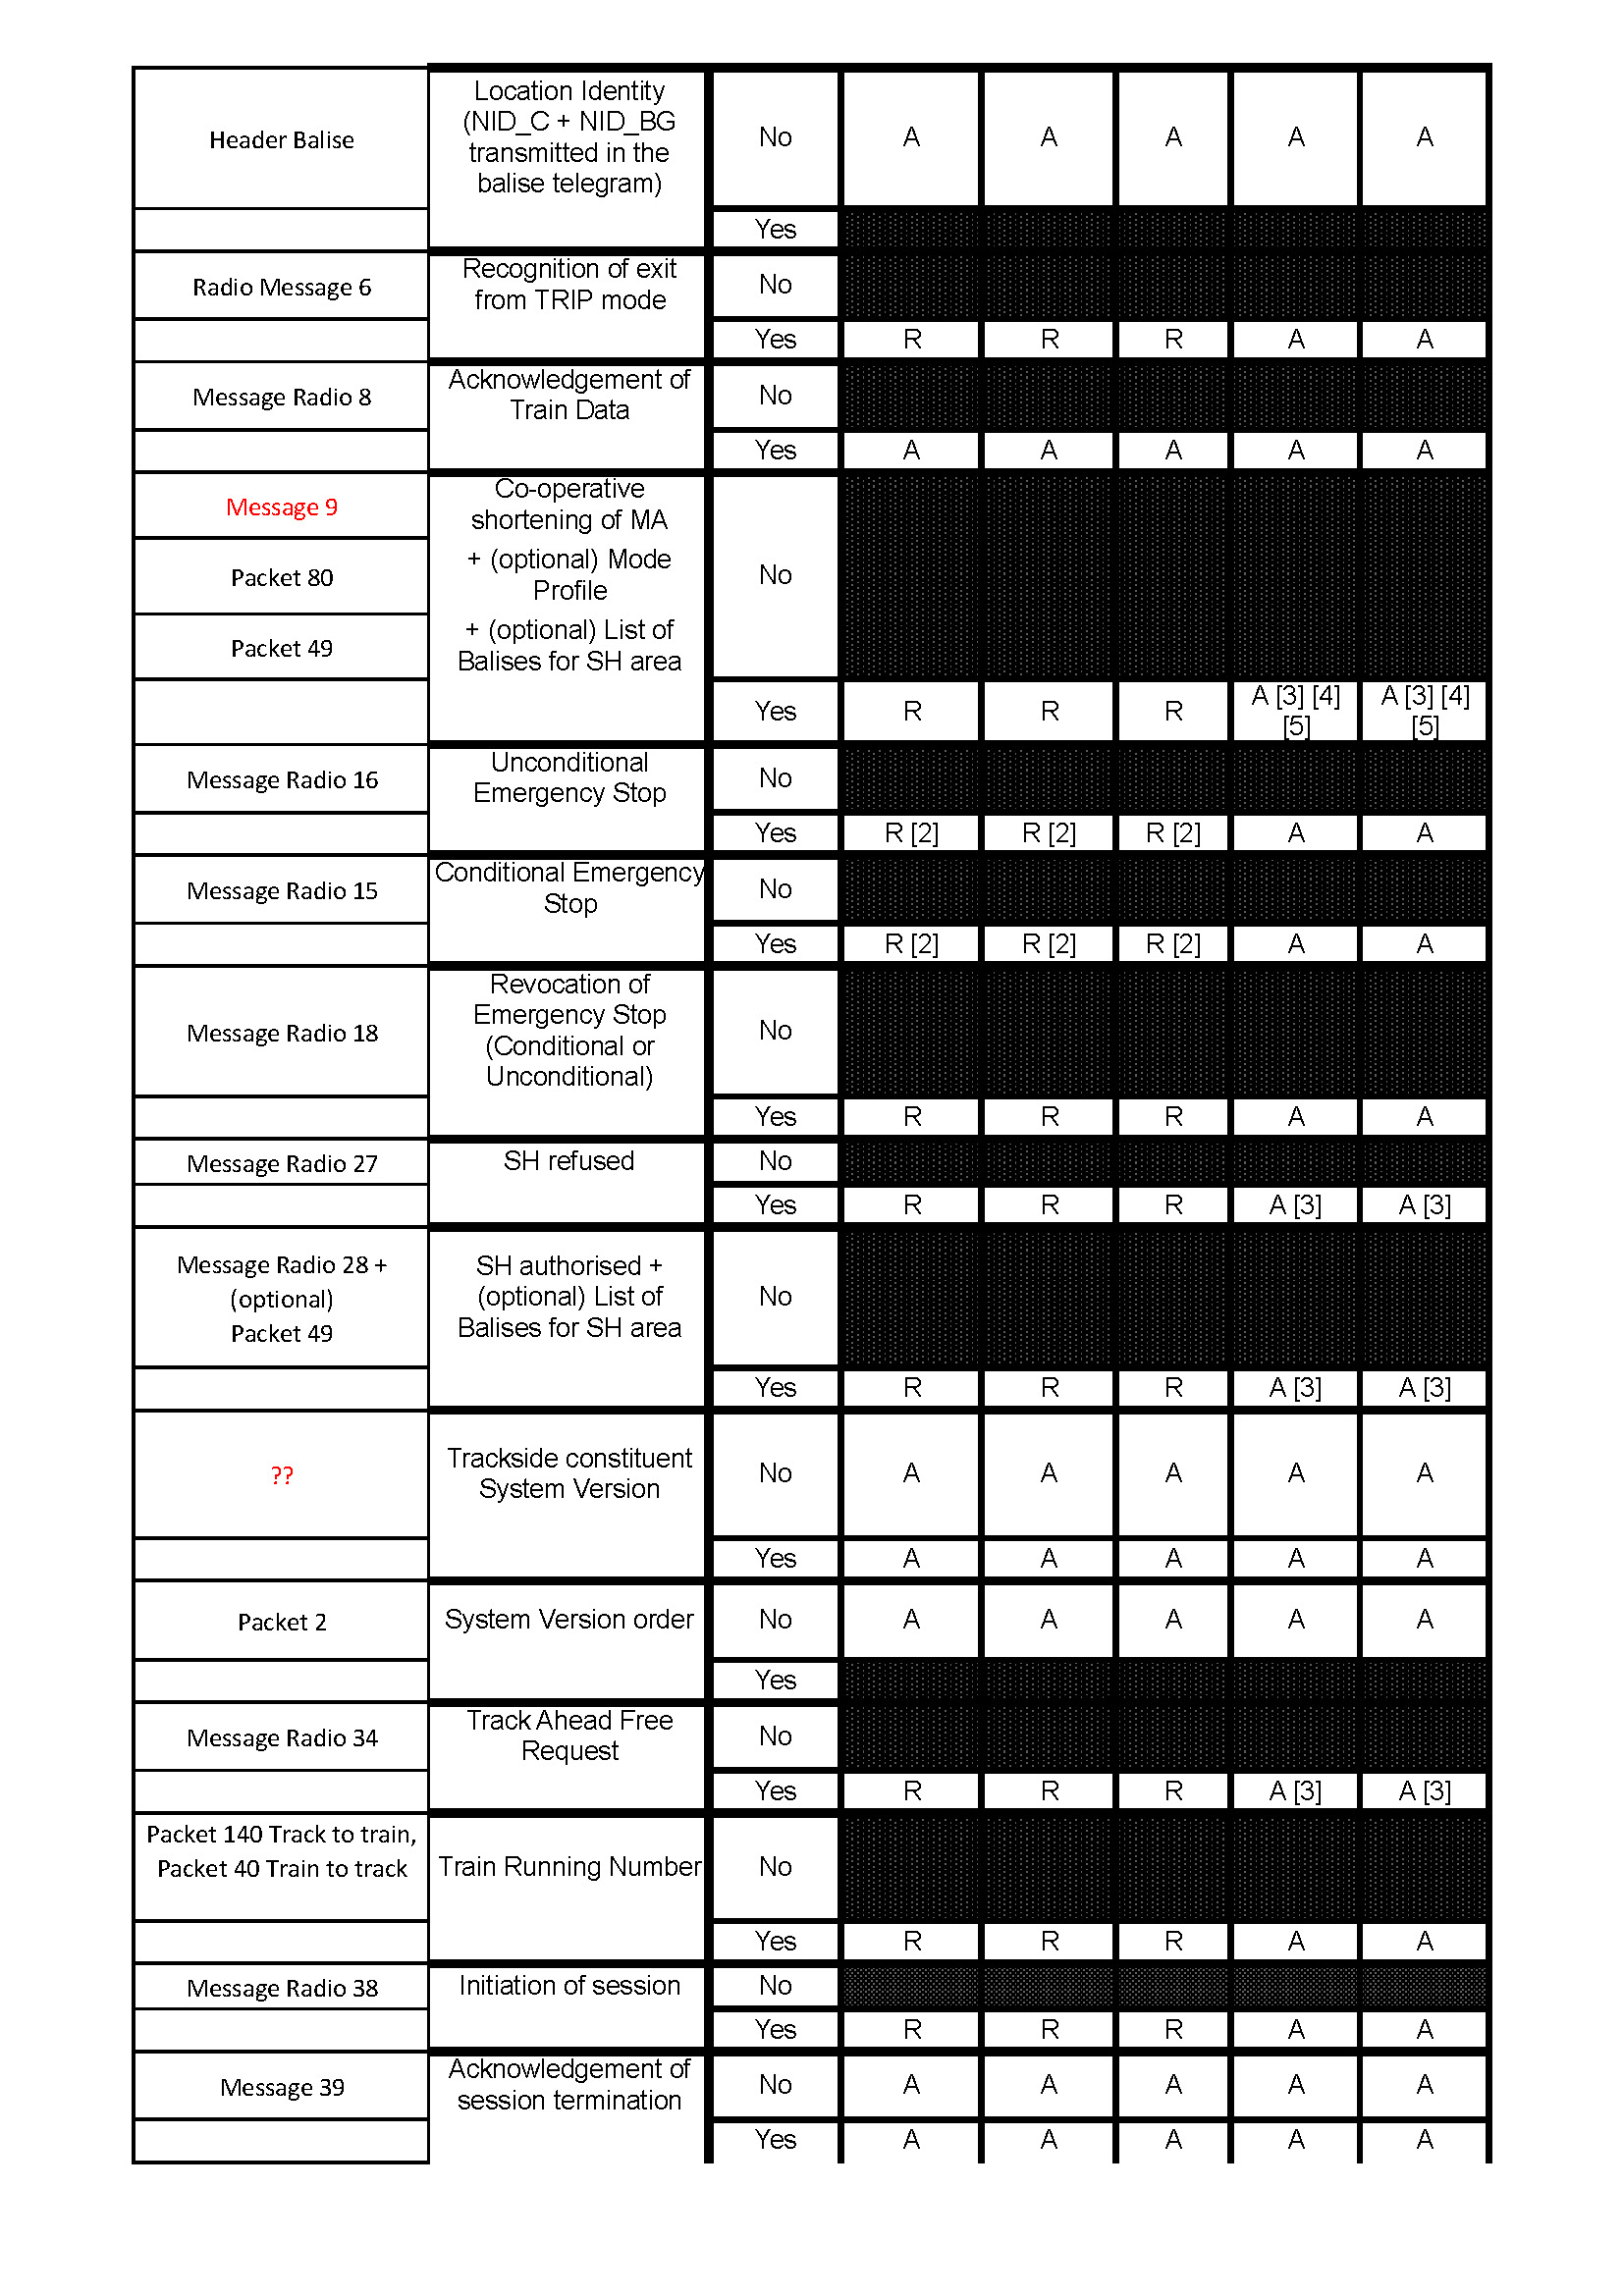
\includegraphics [scale=0.6]{images/LevelFilter3}
\end{figure}
\begin{figure}[hbtp]
\centering
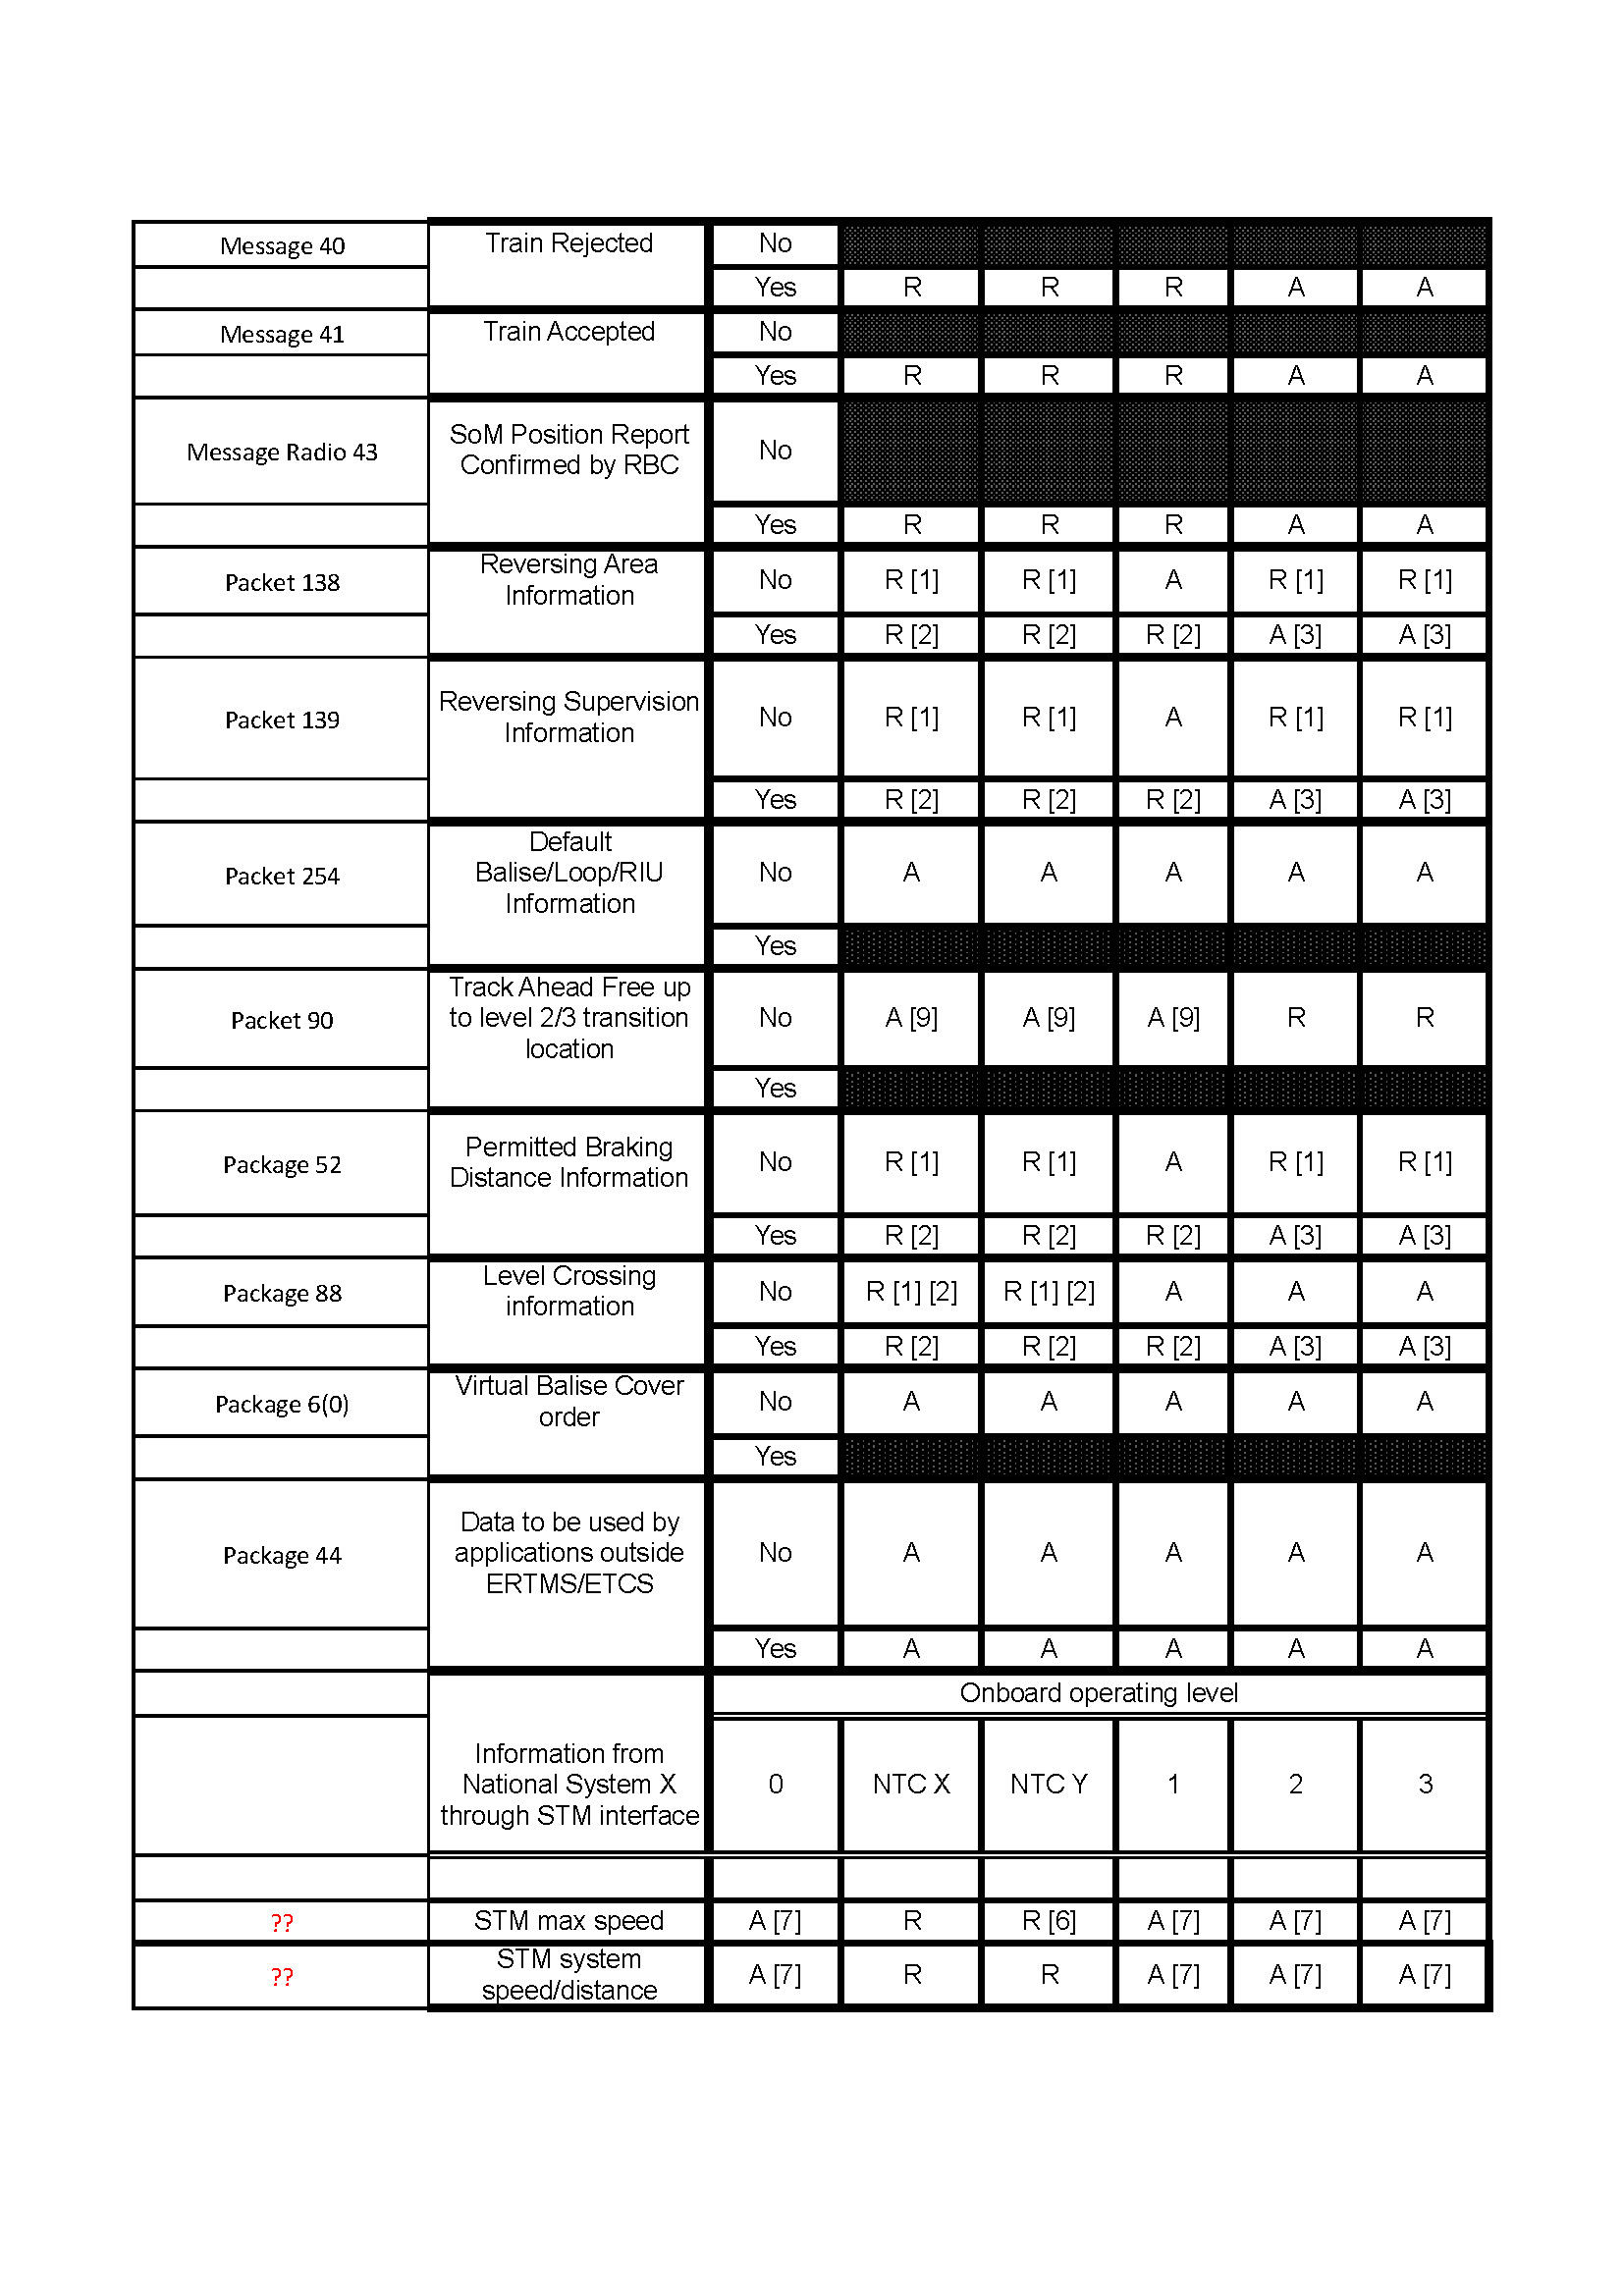
\includegraphics [scale=0.6]{images/LevelFilter4}
\caption{Level Filter}
\end{figure}
\newpage

\paragraph{Filter on Modes}
\begin{figure}[hbtp]
\centering
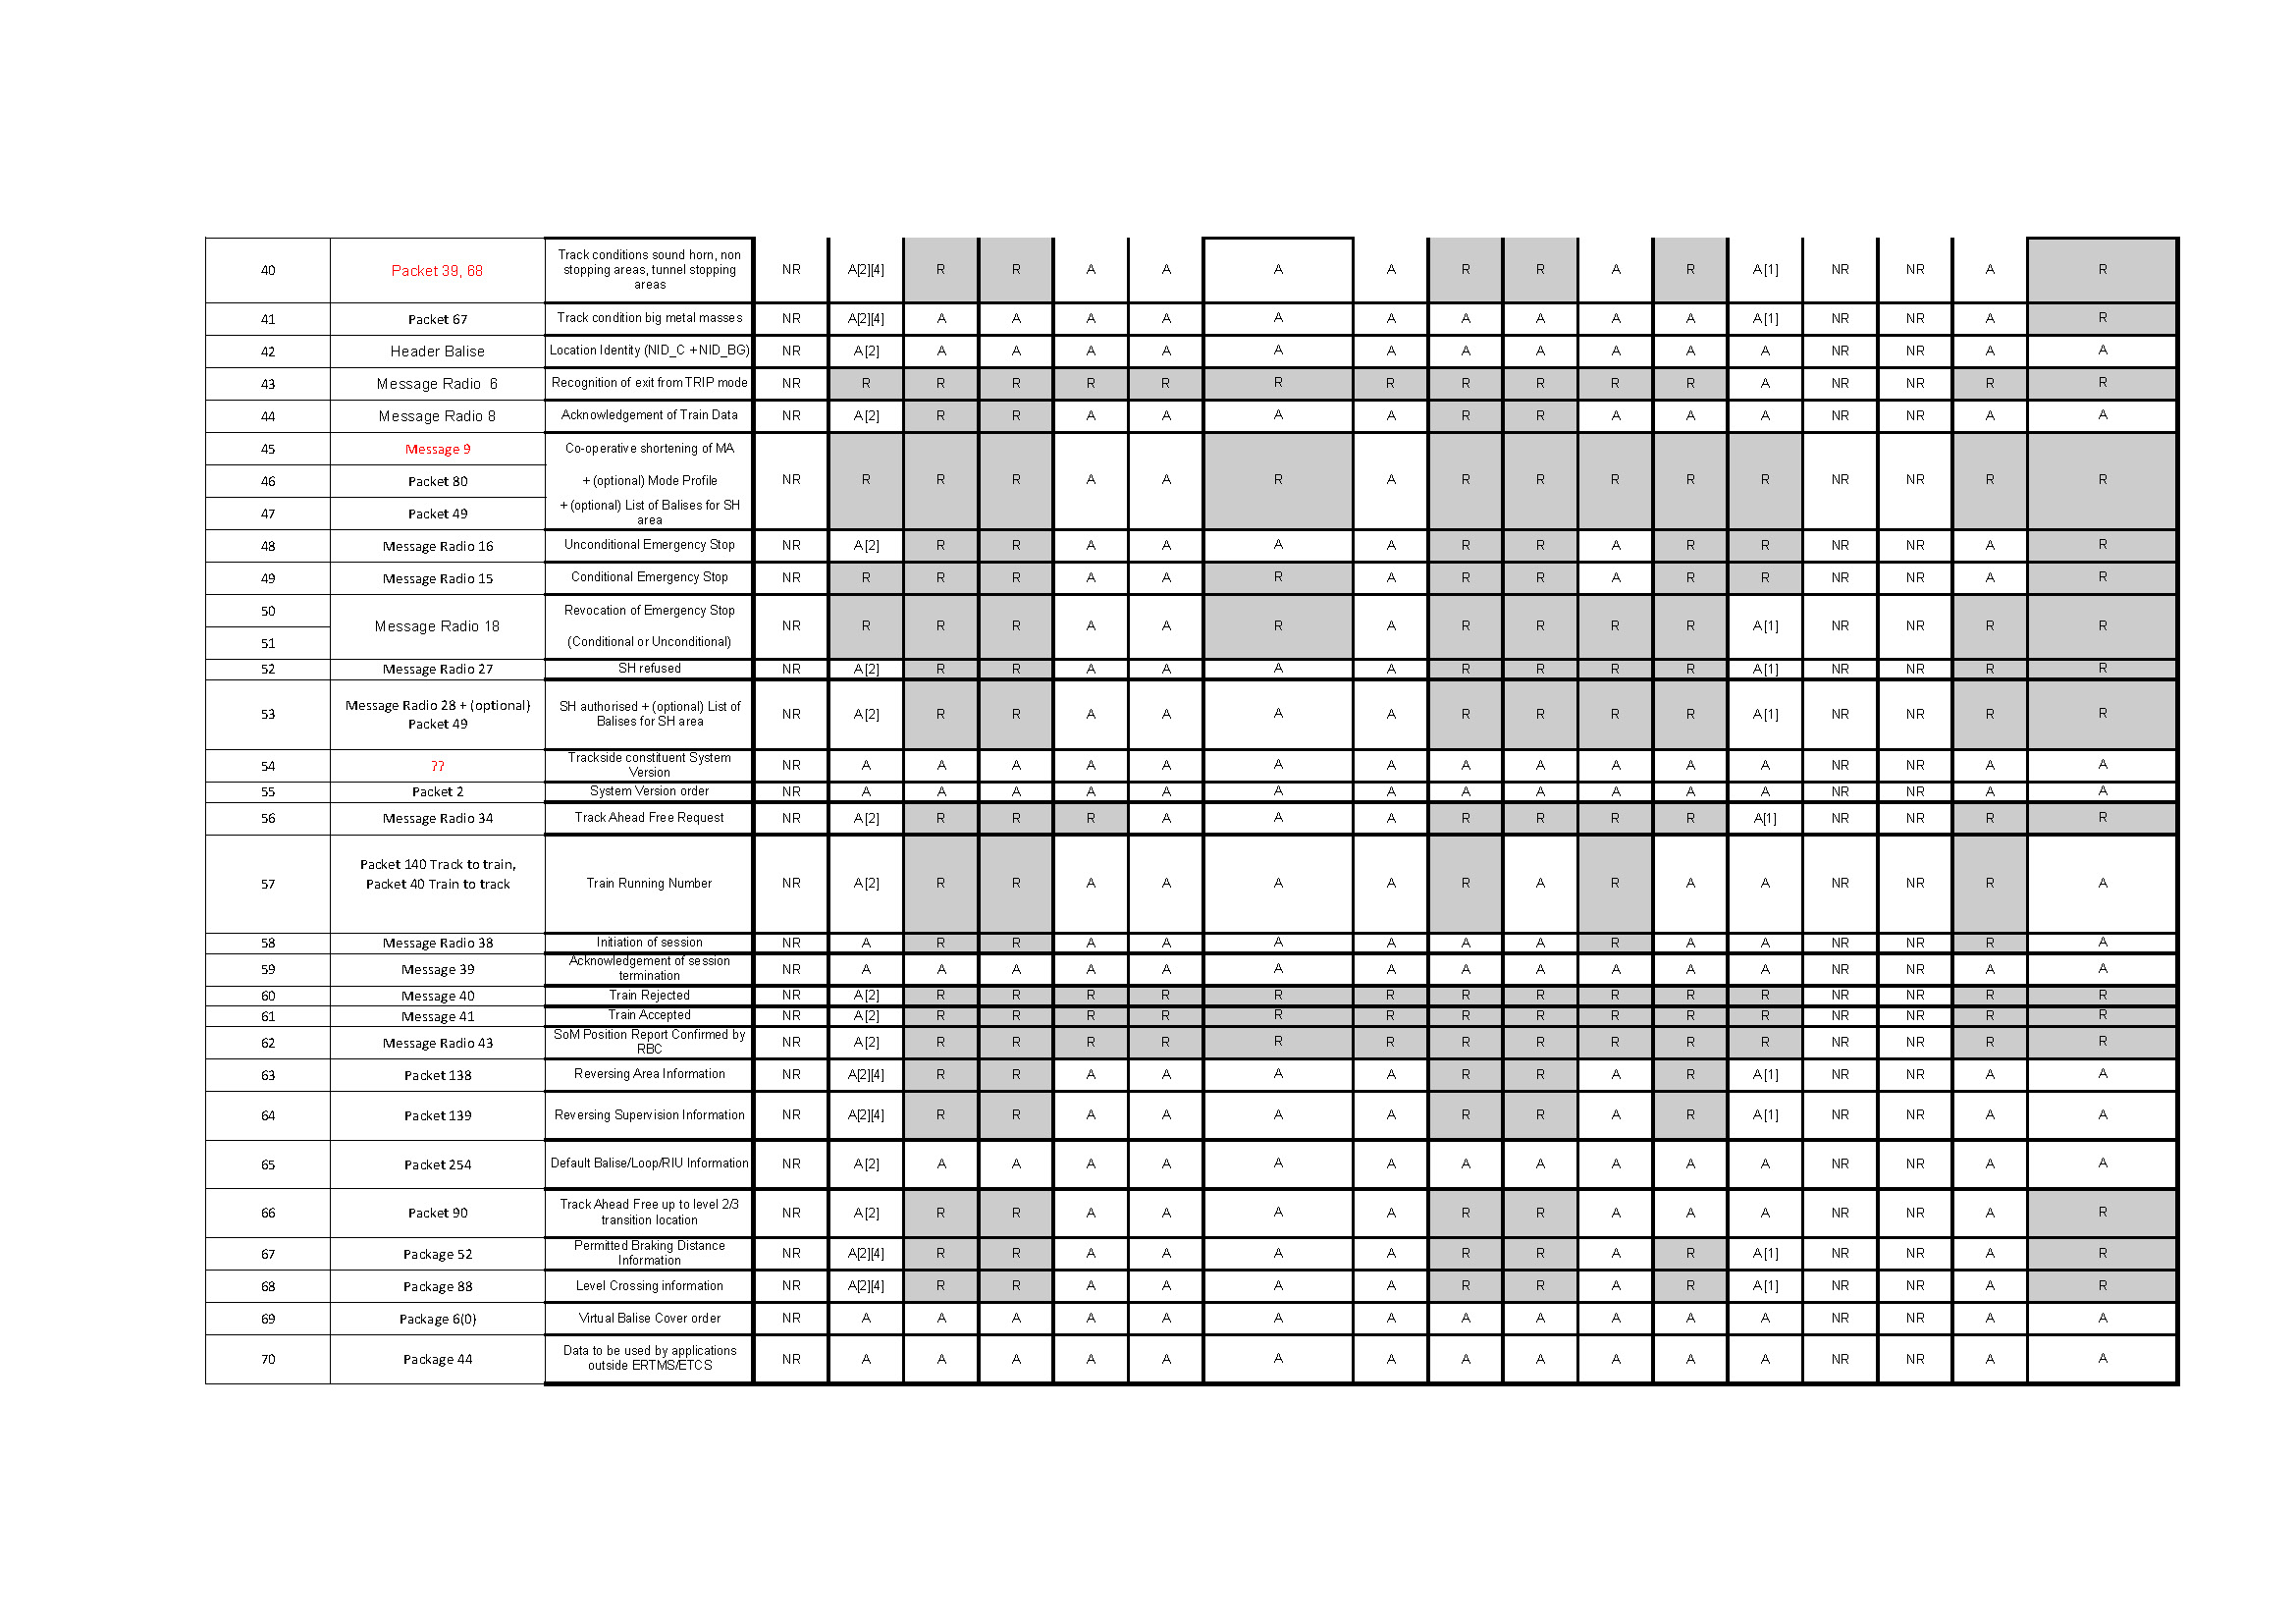
\includegraphics [angle=90, scale=0.8]{images/FilterMode1}
\end{figure}
\begin{figure}[hbtp]
\centering
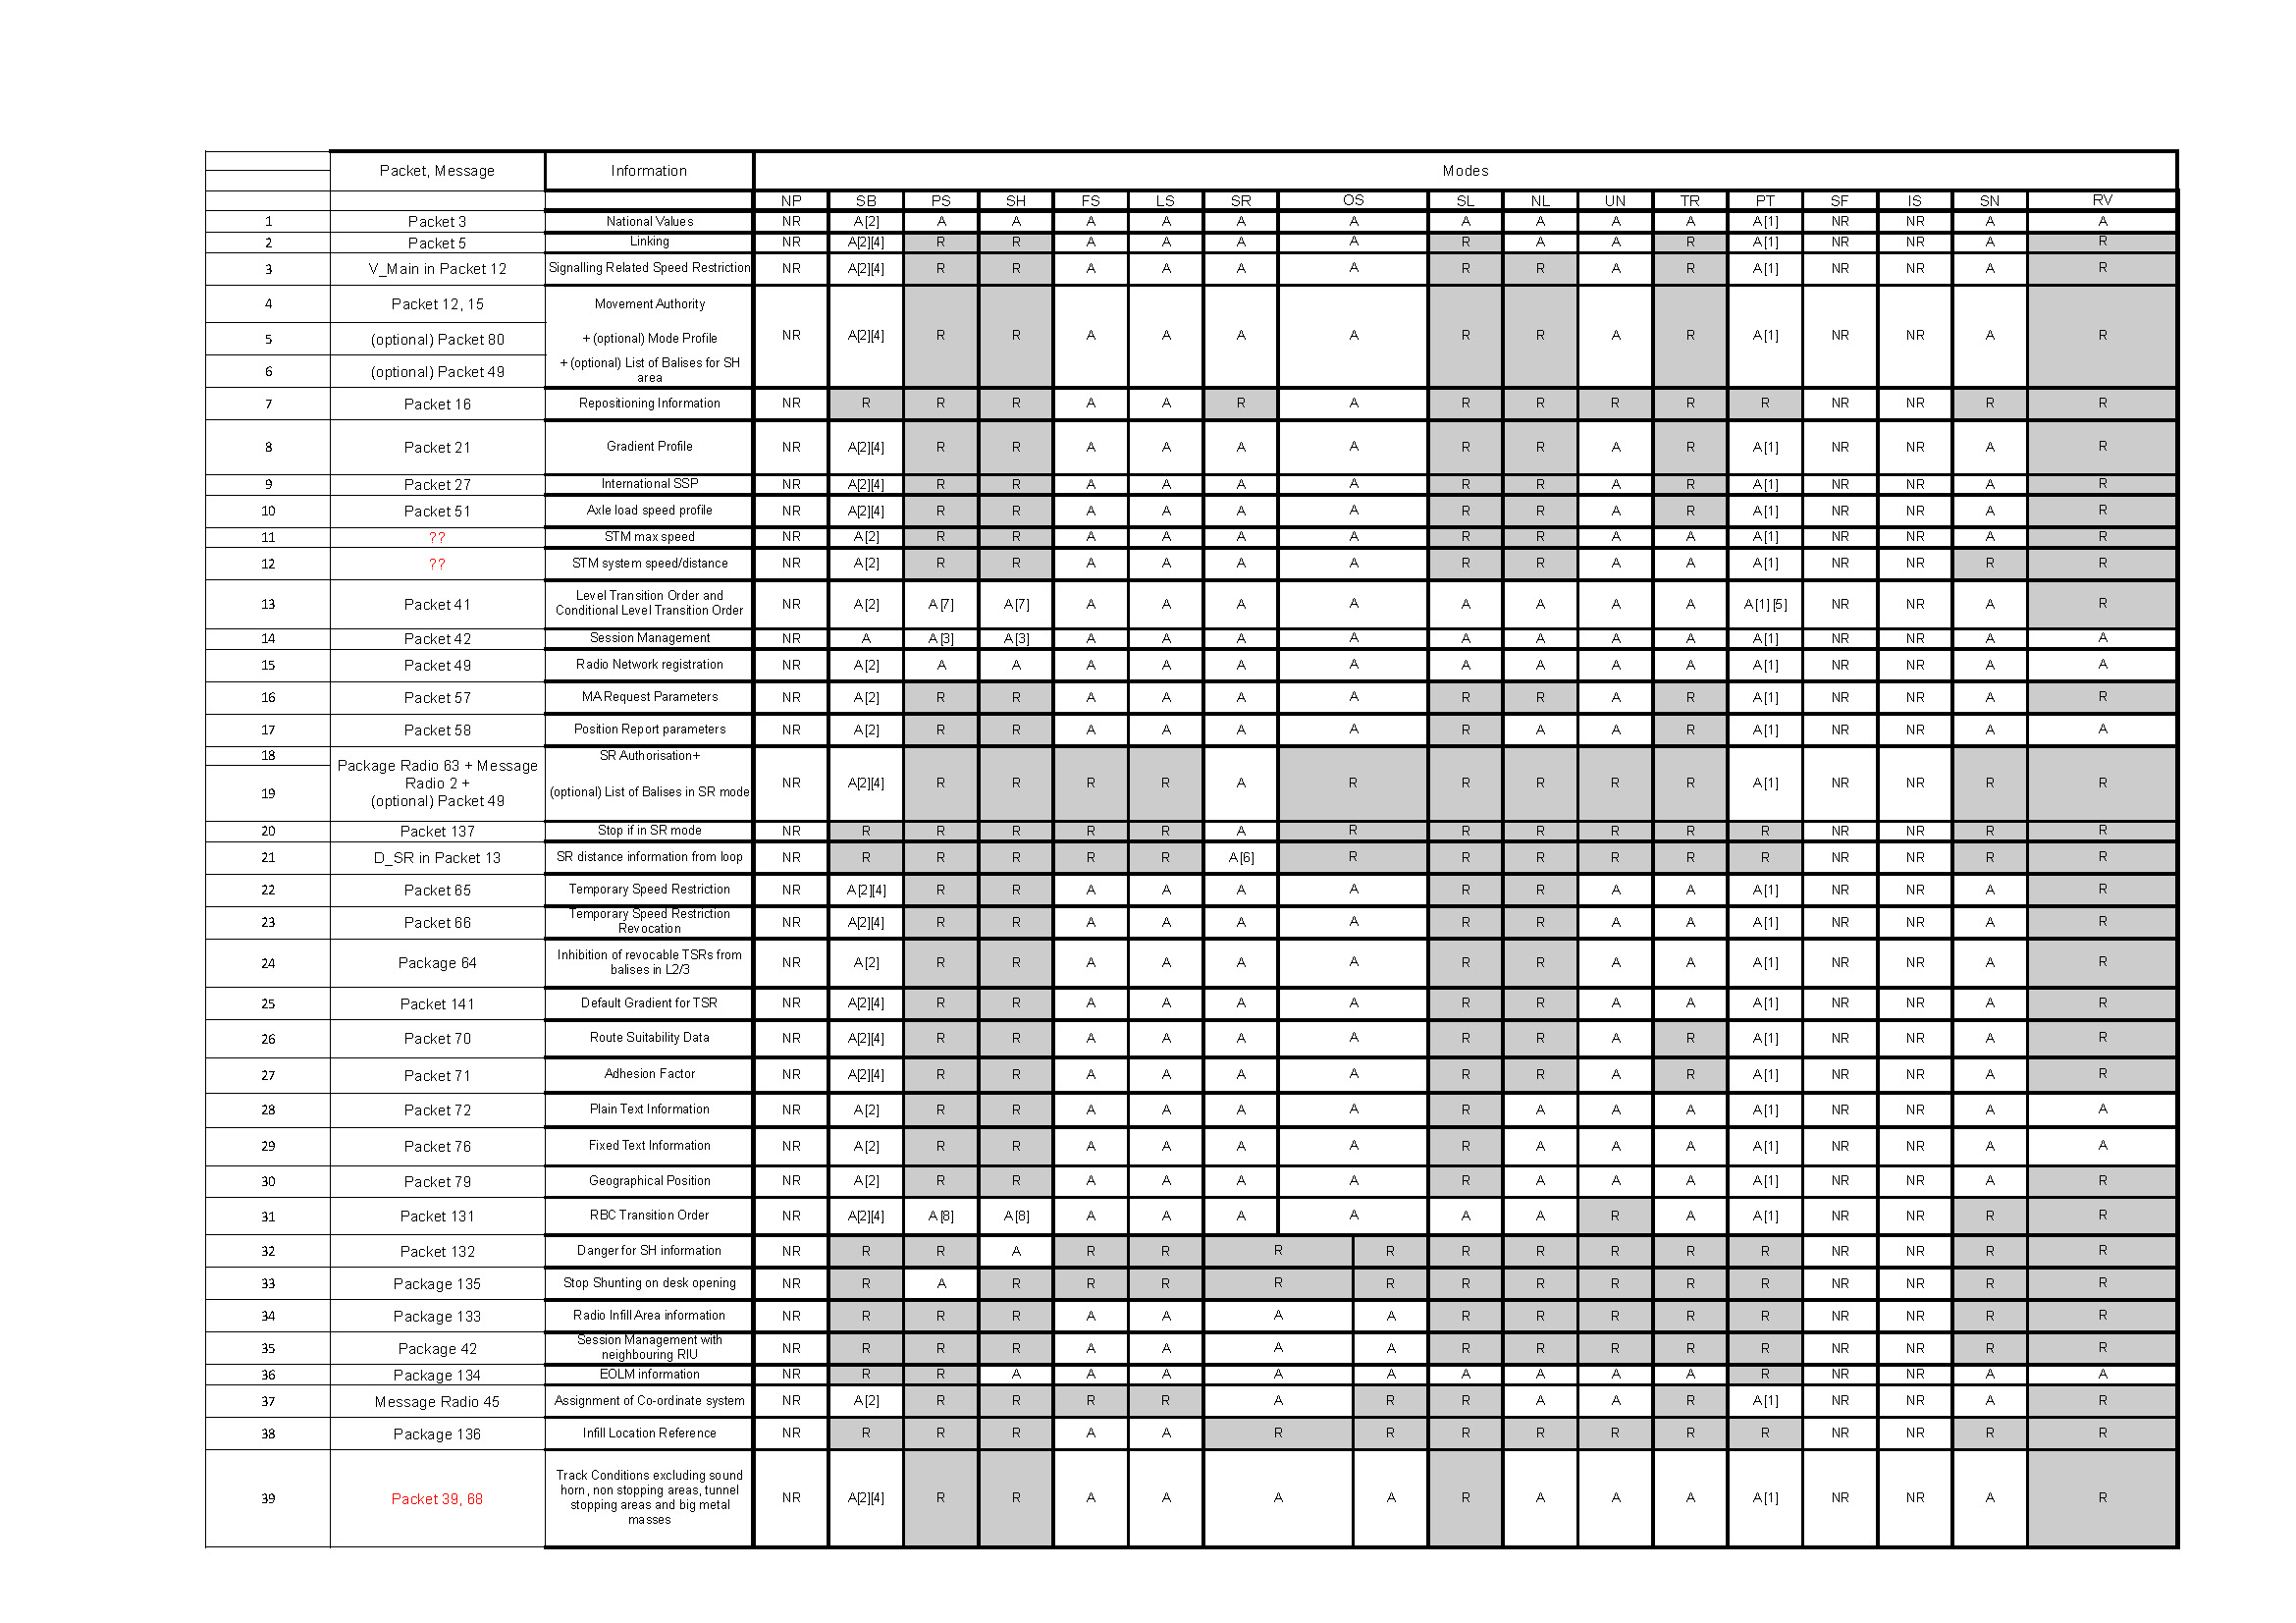
\includegraphics [angle=90, scale=0.8]{images/FilterMode2}
\end{figure}
\begin{figure}[hbtp]
\centering
\caption{Mode Filter}
\end{figure}
\newpage





\paragraph{Filtering (Mode/Level) - One packet per type}
\textbf{ISSUE: HOW MANY PKT 44, 65 AND 66 PER MESSAGE ARE MAXIMALLY SUPPORTED? (BH: who made this comment??)}\\

- Check on announced and immediate level transition orders in the messages to be filtered (needed for further criteria for filtering, to decide if the data shall be stored in the transition buffer).\\
- Filter data stored in the transition buffer according to the current level (what to do if similar information is available in the new message??). Data can be rejected, accepted or kept in the transition buffer.
(Filtering according to new level will be done directly afterwards in the next cycle)\\
- Filter new received messages according to the current level (new level will be done in the next cycle as according to \gls{SRS} data first has to be filtered according to old level and afterwards to new level). Data can be rejected, accepted or stored in the transition buffer.\\
- Filter (level) accepted data according to originating RBC (supervising or other). Information from \gls{BG}'s, loops or RIU is not filtered with this filter.\\
- Filter (level and RBC) accepted data according to the current mode (only reject or accept)\\


%BH-Input-Old-END

\subsection{Build coordinate system and calculate train position}
%BH-Input-Old-START

- Update the coordinate system when a new \gls{BG} is detected (taking into account detected “balise 1” from not completed \gls{BG}'s), i.e. backward -   - Calculation of position of passed \gls{BG}'s.\\
- Management of multiple detected \gls{BG}'s\\
- Relate the (location based) information in received messages to the reference system\\
- Update train position at LR\gls{BG}\\
- Update the train position with the distance driven since last update (or reset to LR\gls{BG} position)\\

\subsubsection{F.2.2 Calculate Train Position}\label{sss:calctrainpos}

\begin{itemize}
\item \textbf{Short Description of Functionality}\\
The main purpose of the function is to calculate the locations of linked and unlinked balise groups (BGs) and the current train position while the train is running along the track. 

\begin{figure}[hbtp]
\centering
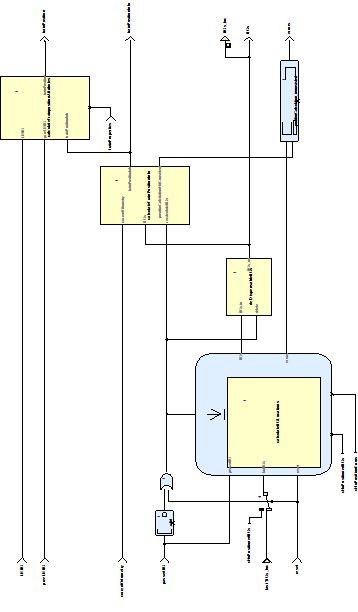
\includegraphics[scale=1]{../images/CalculateTrainPosition.png}
\caption{Structure of calculateTrainPosition}
\end{figure}


\paragraph{Functional Structure in Stages}
The whole function calculateTrainPosition is subdivided into the following steps, which are performed sequentially: 
\begin{enumerate}
\item \textbf{\textit{calculateBGLocations}}: Calculate the balise group locations\\
The first stage is triggered each time the train passes a balise group (input \textit{passedBG}). It takes the balise group header with the BG identification, the linking information (Subset 26, packet 5) and the current odometry values as inputs and calculates the location of the the passed balise group. If the passed BG has been announced via linking information previously, it takes into account the linking as well as the odometry information. If the passed BG does not meet the tolerance window announced by linking, an error flag is set. If the passed BG is an unlinked BG, its location is determined by odometry only, but related to the next previously passed linked BG, if there is one.\\
Then, if the passed BG is a linked BG comprising linking information for BGs ahead, the linking information is evaluated by creating the announced BGs and computing their locations from the linking distances.\\
The passed and the announced BGs are stored in a list \textit{BGs}, ordered by their nominal location on the track.\\
Afterwards the locations of all BGs are further improved by re-adjusting their locations with reference to the just passed BG. This optimizes the BG location inaccuries around the current train position (= location of the passed BG). 

\item \textbf{\textit{delDispensableBGs}}: Delete dispensable balise groups\\
The second stage removes balise groups supposed not to be needed any longer from the list of \textit{BGs}.\\
If the number of stored passed linked BGs exceeds the maximum number of eight as specified in subset-26-3.6.2.2.2 c), all BGs astern are deleted.
If only (passed) unlinked BGs are in the list and exceed the number of \textit{cNoOfAtLeast\_x\_unlinkedBGs}, all passed BGs astern to those are removed from the list. 

\item \textbf{\textit{calculateTrainPositionInfo}}: Calculate train position information.\\
This stage take the list of stored BGs and the current odometry values as inputs and steadily provides the current train position. 

\item \textbf{\textit{calculateTrainpositionAttributes}}: Calculate train position attribute information.\\
This stage provides several additional position related attributes that might conveniently be used by subsequent consumers in the architecture. It requires the actual LRBG and the previous LRBG to be assigned external from the list \textit{BGs}. 

\end{enumerate}

\item \textbf{Reference to the SRS (or other requirements)}\\
\\
The component calculateTrainPosition determines the location of linked and unlinked balise groups and the current train position during the train trip as specified mainly in subset-026-3.6

\item \textbf{Design Constraints and Choices}\\
\\
The following constraints and prerequisites apply:

\begin{enumerate}
\item The input data received from the balises groups must have been checked and filtered for validity, consistency and the appropriate train orientation before delivering them to calculateTrainPosition. 
\item The storage capacity for balise groups is finite. calculateTrainPosition will raise an error flag when a balise group cannot be stored due to capacity limitations.
\item calculateTrainPosition will raise an error flag if a just passed balise group is not found where announced by linking information. It will not (yet) detect when an announced balise group is missing. 
\item calculateTrainPosition is not yet prepared for train movement direction changes. 
\item calculateTrainPosition does not yet consider repositioning information.
\end{enumerate}

\end{itemize}

\subsubsection{Provide Position Report}\label{sss:provposrep}

\begin{figure}[ht]
\centering
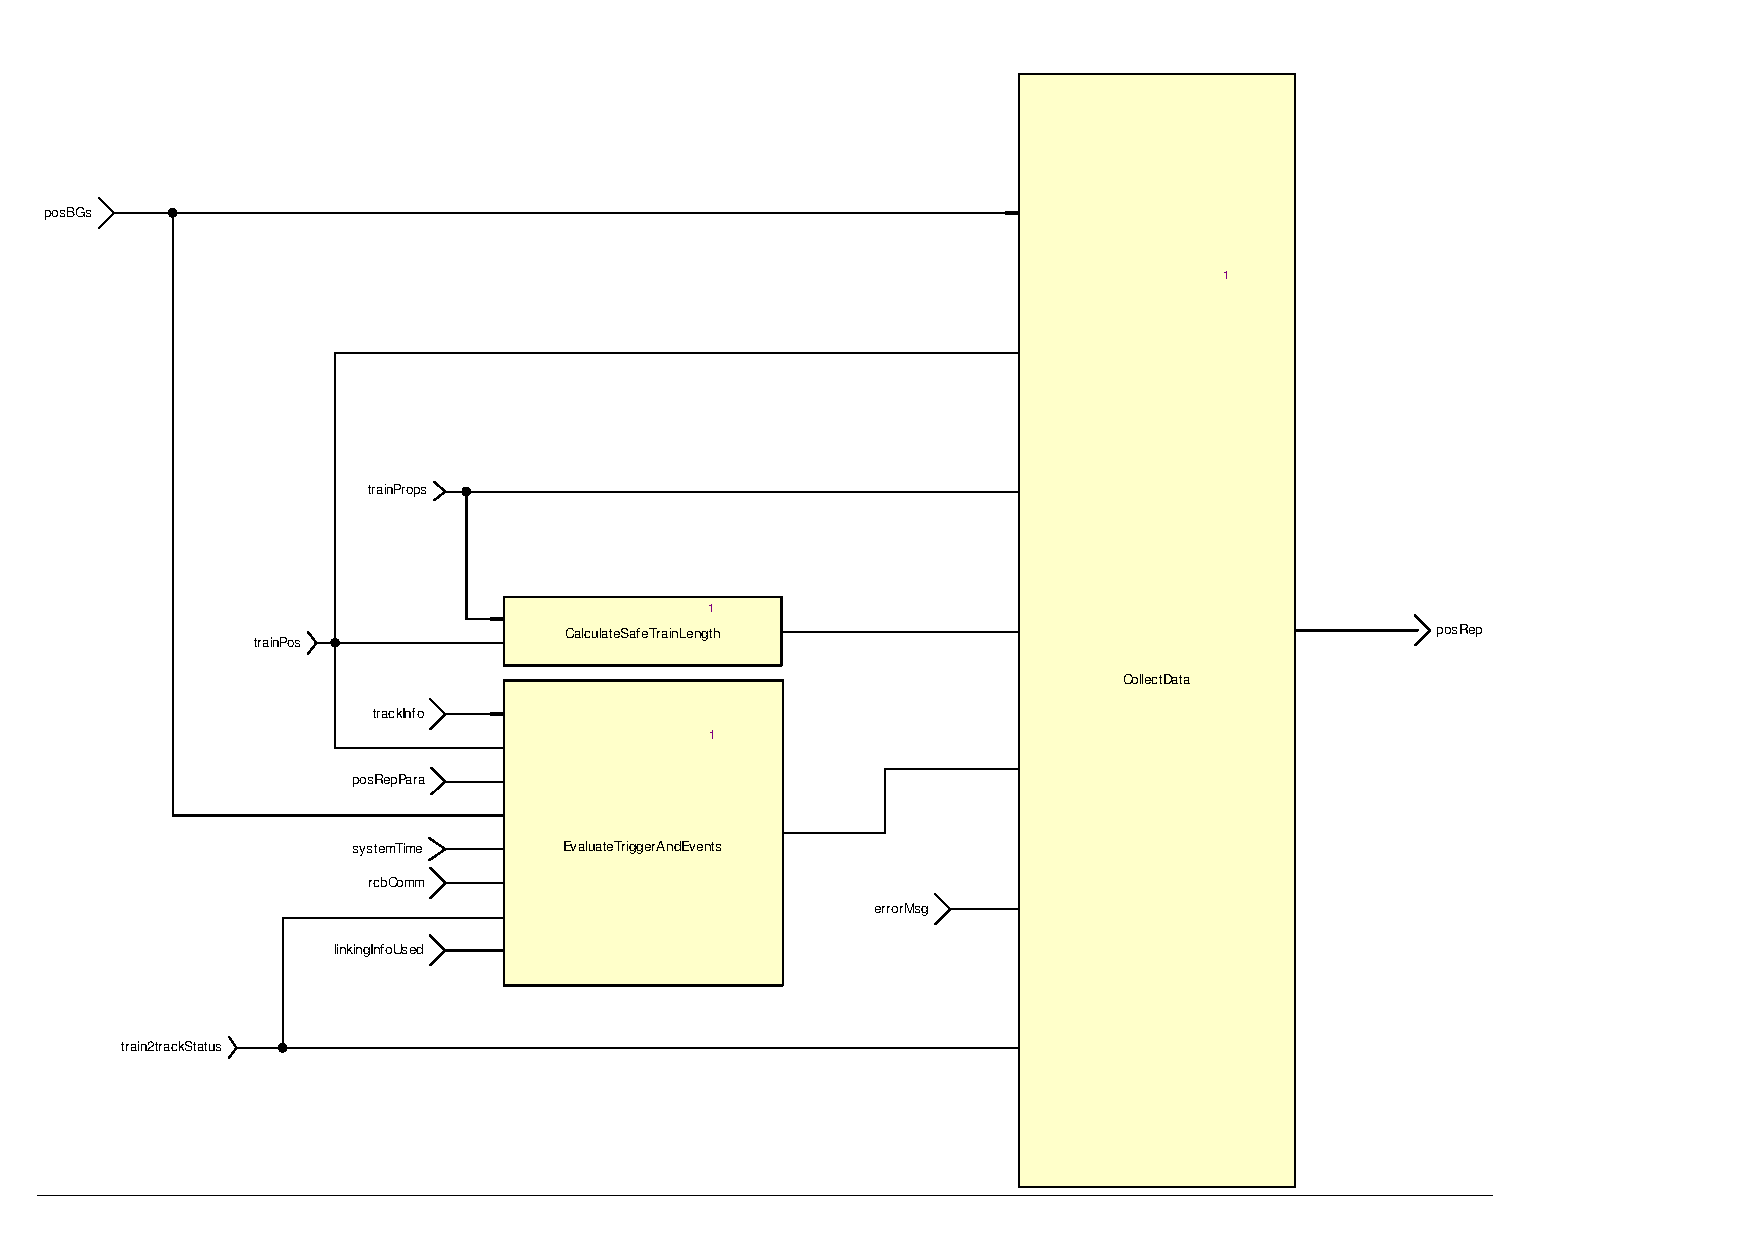
\includegraphics[scale=0.6]{../images/ProvidePositionReport.pdf}
\caption{Structure of component ProvidePositionReport}\label{fig:provideposrep}
\end{figure}

\begin{itemize}
\item \textbf{Short Description of Functionality}\\
This function takes the current train position and generates a position report which is sent to the RBC. The point in time when such a report is sent is determined from event, on the one hand, and position report parameters---which are basically triggers---provided by the RBC or a balise group passed, on the other hand. The functionality is modeled using three operations, as shown in Fig.~\ref{fig:provideposrep}, which are explained below.
\begin{description}
	\item[CalculateSafeTrainLength] Calculates the the safeTrainLength according to Chapt.~3.6.5.2.4/5.
\verb+safeTrainLength = absolute(EstimatedFrontEndPosition - MinSafeRearEnd)+, where
\verb+MinSafeRearEnd = minSafeFrontEndPosition - L_TRAIN+
	\item[EvaluateTriggerAndEvents] Returns a Boolean modeling whether the sending of the next position report is triggered or not. It is the conjunction of the evaluation of all triggers (PositionReportParameters, i.e., Packet 58) and events (see Chapt.~3.6.5.1.4).
	\item[CollectData] In this operation, data of Packet0, \dots, Packet5 and the header is aggregated to a position report.
\end{description}
\item \textbf{Reference to the SRS (or other requirements}\\
Most of the functionality is described in subset 26, chapter~3.6.5.
\item \textbf{Design Constrains and Choices}\\
\begin{enumerate}
	\item The message length (i.e., attribute \verb+L_MESSAGE+) is by default set to 0; the actual value will be set by the Bitwalker/API.
	\item The attribute \verb+Q_SCALE+ is assumed to be constant; that is, all operations using this attribute do not convert between different values of that attribute.
	\item \textit{PositionReportHeader}: The time stamp (i.e., attribute \verb+T_TRAIN+) is not set; this should be done once the message is being sent by the API
	\item \textit{Packet4}: When aggregating the data for this packet, an error message might be overwritten by a succeeding error message. Because the specification only allows to sent one error in one position report, errors are not being stored in a queue, for instance.
	\item \textit{Packet44}: This packet is currently not contained in a position report as it is not part of the kernel functions.
	\item The usage of attributes \verb+D_CYCLOC+ and \verb+T_CYCLOC+ as part of the triggers specified by the position report parameters (i.e., Packet 58 sent by the RBC) may lead to unexpected results if a big clock cycle together with small values for the attributes is used. The cause is that the current model increments at every clock cycle the reference value for the distance and time by at most \verb+D_CYCLOC+ and \verb+T_CYCLOC+, respectively and not a factor of it.
\end{enumerate}
\item \textbf{Open Issues}
\begin{enumerate}
	\item Operation \textit{EvaluateTriggerAndEvents} currently ignores parameters \verb+N_ITER+, \verb+D_LOC+ and \verb+D_LGTLOC+ which allow to specify up to 32 position at which a report has to be sent. The positions are relative to the location of a reference balise group. If the RBC sends packet 58, then it also provides a reference balise group; otherwise, if packet 58 is sent by a balise group, then this balise group serves a the reference balise group. Possible realisation in the model: Extend in the interface posRepPara (i.e., Packet 58) by a \verb+NID_BG+ referring to the reference balise group. Am assumption would be that this BG can be found in the list of passed balise group provided by \textit{CalculateTrainPosition} in Sect.~\ref{sss:calctrainpos}.
	\item The specification requires to store the last eight balise groups for which a position report has been sent (see 3.6.2.2.2.c).
	\item For all reports that contain Packet 1 (i.e., report based on two balise groups), the RBC sends a coordinate system. It is unclear where this has to be stored (i.e., somehow the balise groups have to be stored in a database which has then to be updated), see 3.4.2.3.3.6. Moreover, such a coordination system can be invalid and then has to be rejected (see 3.4.2.3.3.7-8). On a more abstract level, we need to think about the interface between the RBC and the OBU or a proper abstraction thereof.
	\item The decision whether a the report consists of packet 0 or packet 1, which is provided in 3.4.2.3.3, is currently not completely modeled. So far, 3.4.2.3.3.1 has only been modeled, thereby assuming ``the last balise group detected'' is the last balise group and not the LRBG. 3.4.2.3.3.2 is unclear. To model 3.4.2.3.3.4 I need information about the last two valid balise groups and the train running direction. This information can be obtained by adding a memory or this information will be provided by \textit{CalculateTrainPosition} in Sect.~\ref{sss:calctrainpos}. Likewise, also 3.4.2.3.3.5 requires knowledge about the last two valid balise groups.
\end{enumerate}
\end{itemize}


\subsection{Store inputs from the TIU}
- Store status inputs (sleeping indicator etc.)\\
- Store changed train data\\
- Store brake status (e.g. in the handling of brake testing).\\
- Store status of on-board systems (for displaying to the driver)\\
- Isolation\\
- Passive shunting\\

\subsection{Store inputs from the \gls{DMI}}
- Store received acknowledgement and inputs in the “\gls{DMI} request buffer” (includes “data-entry”)\\

\subsection{Store data (direct orders, \gls{BG} lists, NV, track data, procedure parameters, confirmations)}
- Store direct and conditional orders\\
- Store \gls{BG} lists for SH and SR\\
- Store National Values, including procedure status information\\
- Store new received track data (version, etc.)\\
- Store procedure parameters\\

\subsection{Update location based data structures}
- Overwrite location based data from a given location on-wards (reference location given in the message)\\
- Insert “Locations” in the data structure, in the order the “Locations” will be passed.\\

\subsection{Manage specific location based data:}
- movement authority (MA) list of sections, message 37, packet 12 (level 1), message 3, packet 15 (level 2), 16 (repositioning, i.e. extending the current section), message 33 (??), packet 70 (route suitability), message 9 (request to shorten MA), packet 90 (track ahead free leads to MA request)    minimum number of elements to be stored: 6\\
- list of announced \gls{BG}'s linking information: packet 5  minimum number of elements to be stored: 30\\
- adhesion factor: packet 71;  only one element\\
- the “gradient profile” (in: pkt 21)  minimum number of elements to be stored: 50\\
- Speed profiles:  packet 27 (SSP)  (the worst case can be determined at reception)\\
- Packet 13	minimum number of elements to be stored: 50\\
- Speed restrictions and non-continuous speed profiles: packet 51 (axle load profile), packet 52 (permitted braking distance), packets 65/66 (TSR), packet 88 (level crossing, incl. stop condition to be reset at standstill). 
minimum number of elements to be stored: TSR: 30, axle load: 30, permitted braking distance:  5 , level crossing: 10. \\
- Reversing area's: packets 138, 139	minimum number of elements to be stored: 1\\
- Mode dependent speeds: message 2  and packet 80  minimum number of elements to be stored: 6\\
- Level transitions: packet 41  minimum number of elements to be stored:  (see ss26, 5.10.1.6): 1\\
- RBC transitions: packet 131\\
- Radio infill area entry or exit: packet 133\\
- Loop announcement: packet 134\\
- \gls{DMI} information: packets 72,76 (text messages), packet 79 (geographical position information), message 34 (track ahead free request)  minimum number of elements to be stored: fixed text: 5, free text: 5, geographical position: \\
- Track conditions (to be passed to the TIU and displayed at the \gls{DMI}): packet 39 (traction system), packet 40 (current limitation),  packet 68 (diverse track conditions), packet 69 (platform conditions). Pkt 139  minimum number of elements to be stored: 20, + 1 for change power supply + 1 for platform conditions, + 1 for current limitation\\
- Route suitability: minimum number of elements to be stored: 3\\
- Big Metal Mass: Technical information (to be used for \gls{BG}-filtering): packet 67 (ignore \gls{BG} integrity)  minimum number of elements to be stored: 5\\
- Virtual balise covers:  minimum number of elements to be stored: 10\\
- list of position report locations. In: pkt. 58  minimum number of elements to be stored: 15\\
- Announced national values.  In: pkt 3 minimum number of elements to be stored: 1
- If new national values are announced, then those can lead to more restrictive braking curves. Therefore a speed restriction has to be calculated for the location where the values become valid, based on the targets in advance of this point. \\

\subsection{Build and update MRSP and list of targets at LR\gls{BG}}
- Overlay speed restrictions (one by one) over the resulting SSP as received from “build location based data”.\\
- Close the resulting profile with the “end of authority” or “limit of authority” as delivered by “MA-management” resulting in the MRSP at the LR\gls{BG}.
(in on-sight or limited supervision mode, those may not be available)\\
- Select list of “speed reductions”\\
- Evaluate (backwards) which targets are relevant, resulting in the list of most restrictive targets at the LR\gls{BG}.\\
- Relocate targets (beyond this location) to the “minimum border crossing location”, i.e. the minimum safe location where National values are changed, and add the minimum resulting speed at this location to the list of targets.\\
- Reasoning:  new national values might cause more conservative braking curves which otherwise could lead to an intervention at the border.\\

\subsection{Profile supervision, i.e. BCM and ceiling speed supervision (active for FS, OS and LS)}
- Update MRSP for distance driven, i.e. lower the distance to all speed decreases with the maximum distance driven since last update, lower the distance to all speed increases with the minimum distance driven since last update, reorder the distances in the list if locations to lower and to increase changed order.\\
- Determine the local maximum speed\\
- Update the list of targets, i.e. lower the distance to all targets with the maximum distance driven since last update (order will not change) and select the current most restrictive target (always the first in the list)\\
- braking curve monitoring; calculate the braking curves to the most restrictive target, taking into account gradients\\
- ceiling speed supervision; monitor against the local maximum speed.\\

\subsubsection{Movement supervision}
- Roll away protection\\

\subsubsection{Area Supervision}
In shunting, post trip, reversing and staff responsible an area (plus in some cases ceiling speed) is protected. In unfitted only a speed. The way the area is protected differs per mode therefore a function shall be available for each mode:\\
- area supervision in shunting (taking into account a list of \gls{BG}'s to be passed)\\
- area supervision in staff responsible (taking into account a list of \gls{BG}'s to be passed and/or a distance)\\
- reversing area supervision\\
- post trip supervision (only reverse movement).\\

\subsubsection{Update procedure status (including commanding actions towards driver, radio or RBC)}
- SoM:\\ 
- EoM\\
- Enter shunting by driver or track side command
override\\
- Enter “on sight”\\ 
- Enter “staff responsible”\\
- level transitions\\
- Manage train trip\\
- Exit shunting\\
- Passive shunting\\
- Change train orientation\\
- Splitting/combining\\
- Stopping in rear of LX level crossing\\
- Changing train data (not by the driver)\\
- Handling track conditions (including indications):  not applicable for Amsterdam-Utrecht\\
- Limited supervision entry:  not applicable for Amsterdam-Utrecht\\
- release brakes (after trip)\\
- handle track ahead free request\\

\subsubsection{Mode/Level management}
- Manage all conditions for level changes except the direct transitions (handled in filtering): F41\\
- Manage all conditions for mode changes (except msg 16 if that leads to a mode change): F42\\

\subsubsection{\gls{DMI} management}
- update the MRSP at the LR\gls{BG} and construct the \gls{DMI} image\\
- collect BCM results\\
- Check displaying of location dependent txt messages\\
- Calculate geographical position based on stored track-km references\\
- Display required ack-requests, T.A.F. requests etc.\\
- Display mode and level information\\

\subsubsection{RBC communication and Radio management}
\textbf{Manage CNX and DCNX Euroradio}

\paragraph{Short Description of the Functionality}
This function will describe the estabilishing of a initialisation or ending of a RBC communication session\\

\paragraph{Reference to the SRS (or other requirements)}
The functionality will be described in the SRS under the §3.5, § 5.15\\

\paragraph{Interfaces}
\textbf{Input from:} Track information: info CNX/DCNX - Package 42 or 131, Version ERTMS/ETCS - Radio Message 32\\

\textbf{Output to:} Information to the Track: Session initalization: Radio Message 155, Session establishet - Radio Message 159, Not compatible version - Radio Message 154\\

\textbf{picture of interface must implemented in the ADD document}

\textbf{SysML/Scade Model}

\textbf{Documentation of design}

 \paragraph{For the ERTMS Onboard it should be possible to establish a Radio communication if}

- In the context of a start of a start of mission: Traindatas.\\

- in the context of a command from the track information - info CNX/DCNX. The command to contact a RBC will include the idendity of the RBC and the contact number (package 42 or 131).\\

\textbf{Steps to initializes a radio session will be described as followed (§ 3.5.3.9.1 Figure 3)}\\

\paragraph{Initalization of Radio Session}
\begin{figure}[hbtp]
\centering
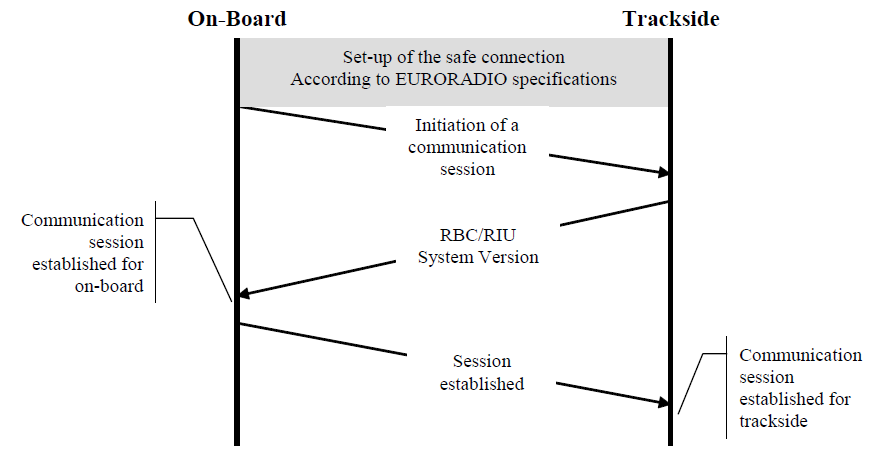
\includegraphics [scale=0.5]{images/startingRBCsession}
\caption{Establishement initiated by on-board (Figure 3 in the SRS 26 § 3.5.3.9.1}
\end{figure}
\newpage


\paragraph{Steps for Establishment of Radio session (§ 3.5.3.1.0. Figure 4)}
- The ERTMS On Board Unit will establish a session through the Euroradio Modul. If necessary the session will repeated (§ 4.3.1.1.).\\

- Function communication will be send to the RBC ``initatio of communication session'' (Radio Message 155).\\

- The RBC must react/acknowledge with the Version ERTMS/ETCS {Radio Message 32}.\\

- The ERTMS Onboard Unit consider the session as established if the ERTMS/Versio is compatible und the Radio Message 159 has been sent to the RBC. The position report report § 3.6.1.5.4 h must be considered.\\

- If the ERTMS/ETCS version is not combatiple with the On Board Unit, the Radio Message 154 ``no compatible version'' must be sent and the session will be declined.\\

- If the Radio Session is established and the sessio is lost by accident, the Euroradio On Board Unit will repeat the the intialization of establishing of a Radio session. During the repeating process the Radio session should be considered as established (§ 4.3.1.1.).\\

-  If the session is failed after repeating of the try of a initalization of a Radio session, the session should be considered as terminated.\\

\paragraph{Establishment of a Radio sessoin}
\begin{figure}[hbtp]
\centering
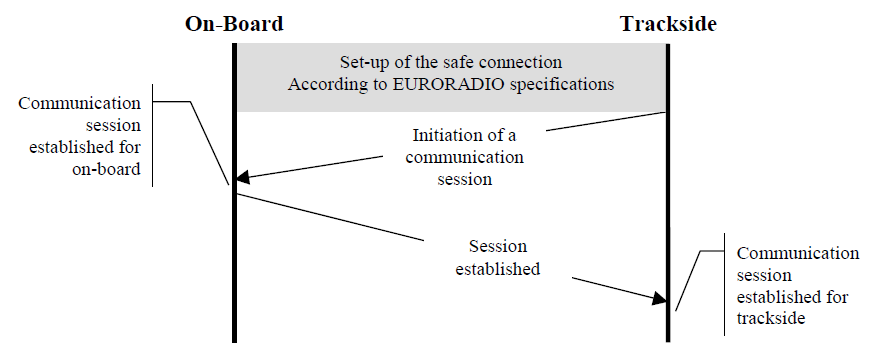
\includegraphics [scale=0.5]{images/EstablishmentofRadioSession}
\caption{Establishement of Radio session (Figure 4 in the SRS 26 § 3.5.3.10.}
\end{figure}
\newpage

\paragraph{Steps to terminate a Radio session (§ 3.5.5.2 Figure 5)}
For the Euroradio it is possible to decline the Radio session if\\

- a message to decline is received from the track (Radio message 156).\\

- After received message ``no compatible version'' (Radio message 154).\\

The idendity of a the ``to connected'' RBC und the Telephonenumber will be include in the activation command or during a RBC/RBC Handover (Package 131 ``establish session to another RBC).\\

- The ERTMS/ETCS On Board Unit will sent the Radio Message ``terminisaiton of commuication session'' (Radio Message 156).\\

- The RBC must an acknowledge to the On Board Unit Euroradio``End of session' (Radio message 39).\\

- After this procedure the the ERTMS/ETCS On Board Unit Eurodio will consider the session as terminated and switch off the Radio Modul.\\

This modul will manage the RBC/RBC Handover.\\
' 
\paragraph{Terminate a Radio session}
\begin{figure}[hbtp]
\centering
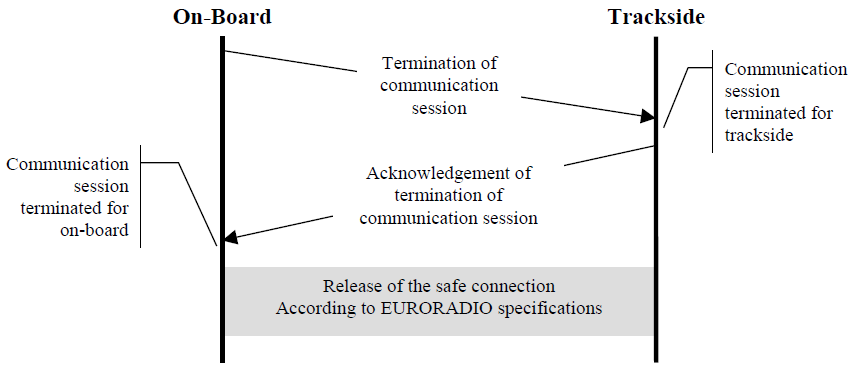
\includegraphics [scale=0.5]{images/TerminationRadiosession}
\caption{Terminate a Radio session (Figure 5 in the SRS 26 § 3.5.5.2}
\end{figure}
\newpage

\subsubsection{RBC/RBC Handover}
\paragraph{Short Description of the Functionality}
The function will manage the RBC/RBC Handover\\
The procedure will be describe in the procedures paragraph\\

\paragraph{Reference to the SRS (or other requirements)}
The functionality will be described in the SRS under the (§ 3.15.1, 5.15)\\

\paragraph{Interfaces}
\textbf{Input from:} information from the Track: RBC ``handover over'' -  package 131, \\

\textbf{Output to:} Information to the Track: ``Position report'' - Radio message 136, \\

\textbf{picture of interface must implemented in the ADD document}

\textbf{SysML/Scade Model}

\paragraph{Documentation of design}
\textbf{ steps during a RBC/RBC handover are as followed if the ERTMS/ETCS On Board Unit consists two GSM-R modems.}\\

\paragraph{MA of ``Handling Over'' - with two GSM-R Modems}
\begin{figure}[hbtp]
\centering
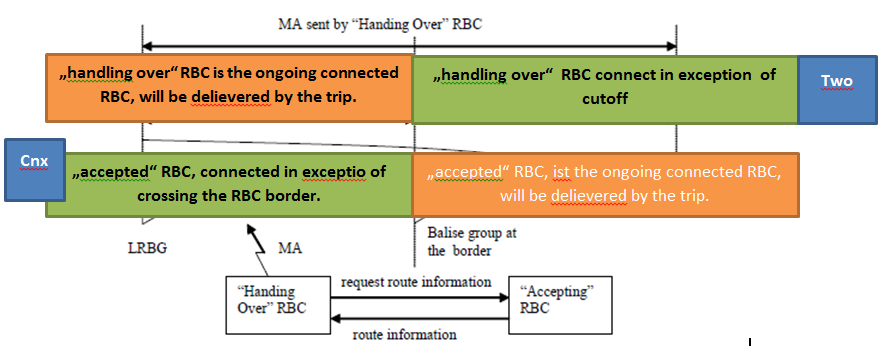
\includegraphics [scale=0.5]{images/Handingover}
\caption{RBC/RBC Handover with two GSM-R modem}
\end{figure}
\newpage

- The ``handling over'' RBC will call the handover on (Package 131.)\\

- The ERTMS/ETCS will establish a communication session with the ``accepted'' RBC\\

- The ERTMS/ETCS On Board Unit will sent a ``position report'' (Radio Message 136) to both RBC´s regarding the max safe front ofthe trasition. The train will be consindered as managed by the ``accepted'' RBC.\\

- The ERTMS/ETCS Onboard Unit will send a ``position report'' (Radio message to both RBC´s within the end of the train on the transition. This will be handled in the SRS § 5.15.2.2.61 and § 3.6.5.1.4.e.\\

- The handling over must request the termination of the session.\\

\textbf{ steps during a RBC/RBC handover are as followed if the ERTMS/ETCS On Board Unit consists one GSM-R modems.}\\

\newpage

\paragraph{MA of ``Handling Over' - with one GSM-R Modems'}
\begin{figure}[hbtp]
\centering
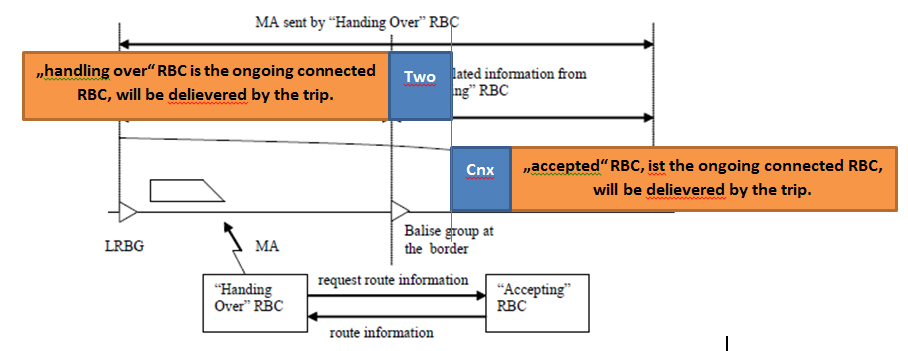
\includegraphics [scale=0.5]{images//Handingover1GSMR}
\caption{RBC/RBC Handover with one GSM-R modem}
\end{figure}
\newpage


Since this handover will be initialized with one Euroradio Modem the proof of the ``handing over'' will be deaktivated tuntil the RBC Handover is accepted with the handover RBC (§ 3.15.1.3.7).\\

- The ``hand over'' RBC will initiated the hand over (Packet 131)\\

- The ERTMS/ETCS On board Unit will send ``position report'' (radio message 136) to the ``handover'' RBC for the RBC border crossing with the datas of the max. head of the train. The same will be done with the end of the train on the transition.\\

- the handling over RBC must initalize the termination of the communication session.\\

- After the session is terminated the ERTMS/ETCS On board Unit will establish a session with the handling over RBC cosider the new RBC as accepted.\\

Every radio session will be sent by the function sent Euroradio messages.\\



- Manage confirmation requests.\\
- Report train position\\
- sent train data for validation\\
- provide acknowledgements on data reception\\

\subsubsection{Sent Radio Messages datas}

\subsubsection{TIU communication}
- Communicate track conditions\\
- Brake test procedure.\\

\subsubsection{JRU and \gls{STM} management: not applicable for Utrecht-Amsterdam}

\newpage

 
\appendix{}

\chapter{Restrictions on Interfaces to openETCS OBU}
The following summarizes restrictions in the scope of implementation of the openETCS OBU. The chosen restrictions are valid for the current scope of the modelling work. They are based on the functions needed to cover the use-case of Utrecht-Amsterdam line.

\section{Track to Train Interface}

Track to Train Interface: Packets Received and The Coverage in openETCS (Section 7.4.1):

\tablefirsthead{
\hline 
\rowcolor{gray} 
Packet Number & Packet Name & Relevant in Scope
\\\hline}
\begin{supertabular}{| p{1,5 cm} | p{10 cm} | p{2,5 cm} |}
0 & Virtual Balise Cover marker & \\\hline
2 & System Version order & \\\hline
3 & National Values & \\\hline
5 & Linking & \\\hline
6 & Virtual Balise Cover order & \\\hline
12 & Level 1 Movement Authority & \\\hline
13 & Staff Responsible distance information from loop & \\\hline
15 & Level 2/3 Movement Authority & \\\hline
16 & Repositioning Information & \\\hline
21 & Gradient Profile & \\\hline
27 & International Static Speed Profile & \\\hline
39 & Track Condition Change of traction system & \\\hline
40 & Track Condition Change of allowed current consumption & \\\hline
41 & Level Transition Order & \\\hline
42 & Session Management & \\\hline
44 & Data used by applications outside the ERTMS/ETCS system. & \\\hline
45 & Radio Network registration & \\\hline
46 & Conditional Level Transition Order & \\\hline
49 & List of balises for SH Area & \\\hline
51 & Axle load Speed Profile & \\\hline
52 & Permitted Braking Distance Information & \\\hline
57 & Movement Authority Request Parameters & \\\hline
58 & Position Report Parameters & \\\hline
63 & List of Balises in SR Authority & \\\hline
64 & Inhibition of revocable TSRs from balises in L2/3 & \\\hline
65 & Temporary Speed Restriction & \\\hline
66 & Temporary Speed Restriction Revocation & \\\hline
67 & Track Condition Big Metal Masses & \\\hline
68 & Track Condition & \\\hline
69 & Track Condition Station Platforms & \\\hline
70 & Route Suitability Data & \\\hline
71 & Adhesion Factor & \\\hline
72 & Packet for sending plain text messages & \\\hline
76 & Packet for sending fixed text messages & \\\hline
79 & Geographical Position Information & \\\hline
80 & Mode profile & \\\hline
88 & Level crossing information & \\\hline
90 & Track Ahead Free up to level 2/3 transition location & \\\hline
131 & RBC transition order & \\\hline
132 & Danger for Shunting information & \\\hline
133 & Radio infill area information & \\\hline
134 & EOLM Packet & \\\hline
135 & Stop Shunting on desk opening & \\\hline
136 & Infill location reference & \\\hline
137 & Stop if in Staff Responsible & \\\hline
138 & Reversing area information & \\\hline
139 & Reversing supervision information & \\\hline
140 & Train running number from RBC & \\\hline
141 & Default Gradient for Temporary Speed Restriction & \\\hline
143 & Session Management with neighbouring Radio Infill Unit & \\\hline
145 & Inhibition of balise group message consistency reaction & \\\hline
180 & LSSMA display toggle order & \\\hline
181 & Generic LS function marker & \\\hline
254 & Default balise, loop or RIU information & \\\hline

\end{supertabular}

\section{TIU Interfaces}
The following information is based on the structure given by the Alstom API.

\subsection{Input to openETCS}

\tablefirsthead{
\hline 
\rowcolor{gray} 
Packet Number & Packet Name & Relevant in Scope
\\\hline}
\begin{supertabular}{| p{1,5 cm} | p{10 cm} | p{2,5 cm} |}
0 & Inputs from train devices & \\\hline
1 & Plain text message & \\\hline
2 & Fixed text message & \\\hline
3 & brake models & \\\hline
4 & Not used & \\\hline
5 & Not used & \\\hline
6 & Test and failure detection & \\\hline
7 & STMs specific behaviour & \\\hline
8 & Specific from MVB (Specific to Alstom implementation) & \\\hline
12 & Diagnostic & \\\hline
13 & Inhibition Level (Specific to Alstom implementation) & \\\hline
\end{supertabular}

\subsection{Output from openETCS}

\tablefirsthead{
\hline 
\rowcolor{gray} 
Packet Number & Packet Name & Relevant in Scope
\\\hline}
\begin{supertabular}{| p{1,5 cm} | p{10 cm} | p{2,5 cm} |}
0 & Commands & \\\hline
1 & Track conditions & \\\hline
2 & Odometric data & \\\hline
3 & Other information & \\\hline
4 & Train type & \\\hline
5 & Track condition change of traction power & \\\hline
6 & Location reference update & \\\hline
7 & Sporadic commands & \\\hline
8 & STMs states & \\\hline
9 & Train information & \\\hline
10 & Doors control section & \\\hline
11 & Track description deletion information & \\\hline
14 & Gradients & \\\hline
\end{supertabular}



\bibliographystyle{unsrt}
\bibliography{architecture}


\newpage
\addcontentsline{toc}{chapter}{Index}
\printindex
%===================================================
%Do NOT change anything below this line

\end{document}
